\chapter{\emph{Re-entrant loop search}}
\section{Introduction}
The identification of re-entrant loop structures present in both the Tmem41b and Atg9 targets prompted an investigation into how prevalent these specific structural features are.  

Historically it was thought that alpha helical transmembrane proteins form helical bundles of parallel/antiparallel helices that cross the membrane in perpendicular orientations. However, as more and more alpha helical membrane proteins were solved, their structures revealed  more complex structural topologies.  One such structural feature possessed by some alpha helical transmembrane proteins is the re-entrant loop.  Rather than entering the membrane orthogonally and leaving the opposite side, the re-entrant loop enters the membrane on one side and then turns back to the same side from which it originated and leaves (Figure \ref{fig:topology}).  Re-entrant loops were initially reported in the early 1990s in the cardiac Na\textsuperscript{+}/Ca\textsuperscript{2+} exchanger \cite{iwamoto1999unique}. Since then re-rentrant loops have been detected in other membrane transporters and channels such as aquaporins \cite{de2001refined}, potassium channels \cite{zhou2001chemistry} and chloride channels \cite{dutzler2002x}. 

\begin{figure}[th!]
    \centering
    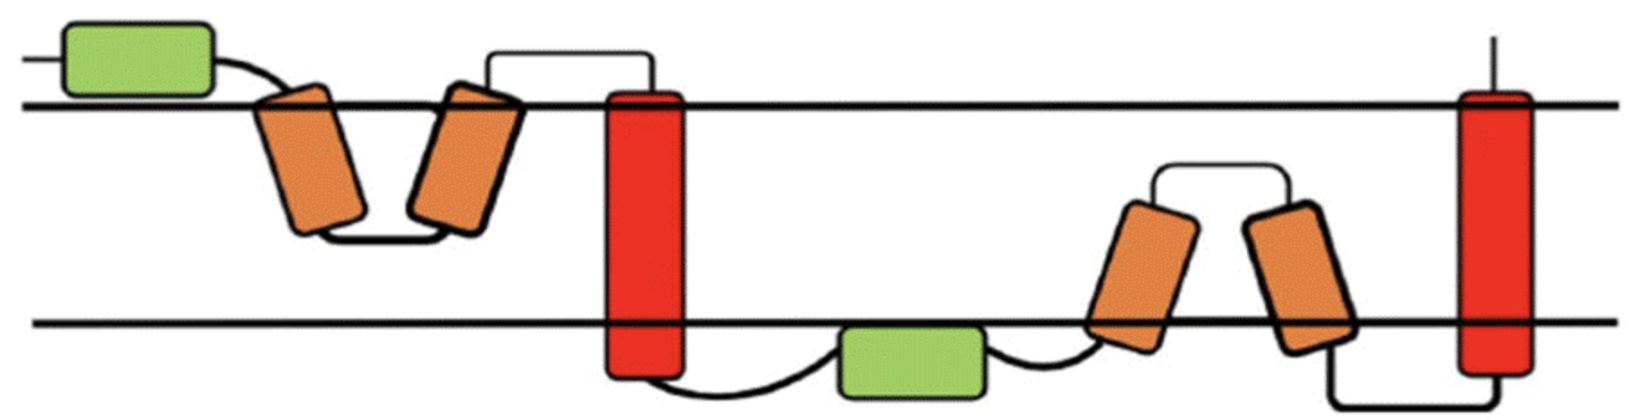
\includegraphics[width=150mm, scale=0.75]{Pfam/topology.png}
    \caption{An inverse pseudo repeat topology showing types of alpha-helical transmembrane structure motifs}
    \label{fig:topology}
    \small
    Green: amphipathic helix, red: transmembrane helix, orange: re-entrant loop.
\end{figure}

Previous studies \cite{Yan2010} have grouped re-entrant loops into three categories. The classification was based on secondary structure distribution along the length of the re-entrant loop.  The re-entrant loops were classed as a helix–coil–helix, helix–coil, coil–helix motifs or regions of entirely of irregular secondary structure \cite{Yan2010}. It has been demonstrated that smaller residues are over represented in re-entrant loops and that the hydrophobicity distribution for re-entrant loops is not symmetric when comparing to transmembrane helices \cite{Yan2010}.  

\begin{figure}[th!]
    \centering
    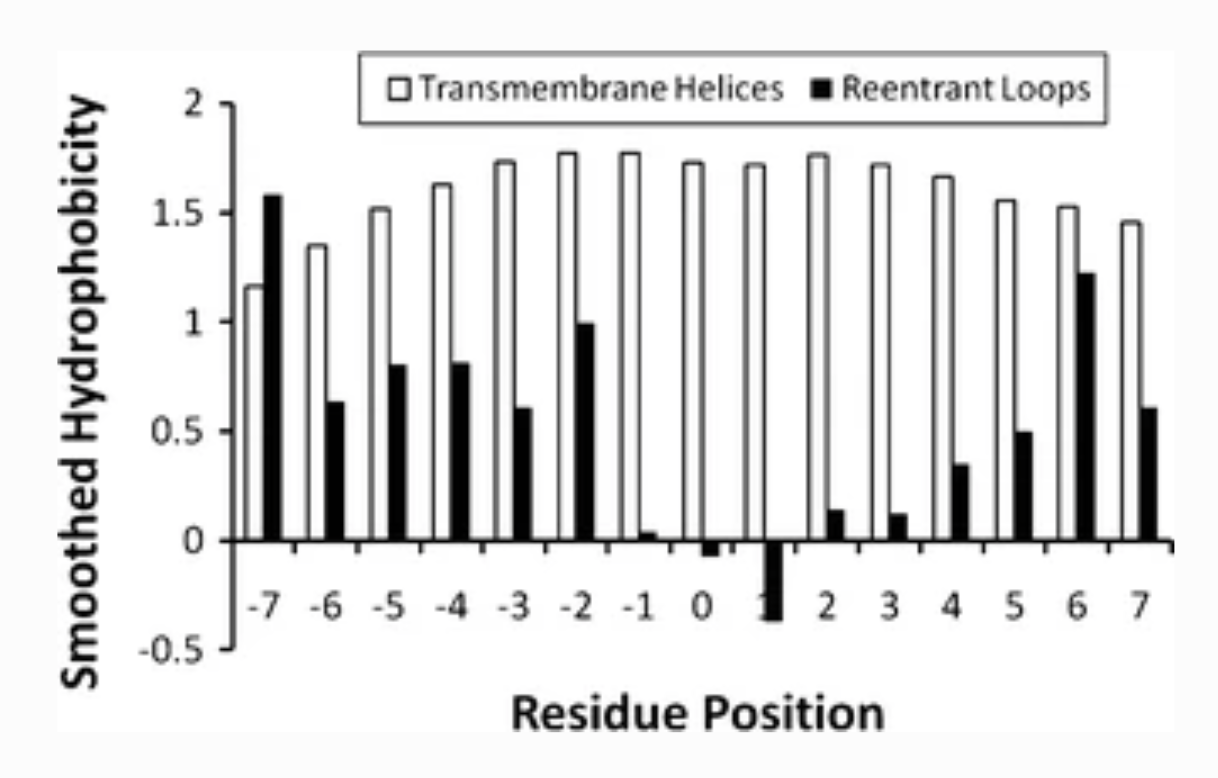
\includegraphics[width=150mm, scale=0.6]{Pfam/re-ent_hydrop_profile.png}
    \caption{Comparison of smoothed hydrophobicity profiles for protein sequences of re-entrant loops and transmembrane helices.}
    \label{fig:hydrophob}
    \small
    Position 0 is the deepest residue embedded in the membrane (adapted from \cite{Yan2010}).
\end{figure}


Sequence methods have been developed which attempted to predict the presence of re-entrant loops utilising hidden Markov models \cite{Yan2010,viklund2006structural}. These methods have been used to predict that more than 10\% of transmembrane proteins contain re-entrant loops and that the their presence increases linearly with the number of transmembrane regions. These studies also indicate that re-entrant loops are most commonly found in channel proteins and least commonly in signal receptors \cite{viklund2006structural}. 

The research into DedA proteins described in chapter 3 predicted that the re-entrant loops present in these proteins form part of an inverse pseudo repeat (Figure \ref{fig:hydrophob}) where they face one another in the membrane with each re-entrant loop in contact with a transmembrane helix.  This architecture has also been highlighted other proteins such as aquaporins \cite{tornroth2010structural}, ion-coupled transporters (where the re-entrant loops are responsible for recognising ions such as Cl\textsuperscript{−} and Mg\textsuperscript{2+}) \cite{forrest2015structural}, and undecaprenyl-diphosphatase (UppP) (where they recognise head groups of phospholipids) \cite{el2018crystal}.  Face-to-face re-entrant loops are also known to recognise small hydrophilic molecules such as uridine and glutamate \cite{forrest2015structural}.  It is common for the re-entrant loops within these structures to possess a highly conserved proline at the turning point (the residue embedded deepest in the membrane) \cite{mesdaghi2020silico} and display an inconsistent hydrophobicity distribution where C-terminal side is more hydrophilic in contrast with transmembrane helices where hydrophobicity distribution is more consistent \cite{Yan2010}. 

The subsequent research into Atg9 revealed the presence of two re-entrant loops with topologies not reported previously.  The high resolution CryoEM structure of human Atg9 was shown to possess four transmembrane helices, and two re-entrant loops (Figure \ref{fig:atg9_pro}).  One re-entrant loop is seen to penetrate far into the membrane with its C-terminal half being parallel to bilayer. The other re-entrant loop is atypically long and the helix extends from the membrane far into the cytosol; this forms a structural scaffold that makes contact with different parts of the oligomer.  The turning points of both re-entrant loops are formed by highly conserved proline residues (Figure \ref{fig:atg9_top})  \cite{guardia2020structure}. 

\begin{figure}[th!]
    \centering
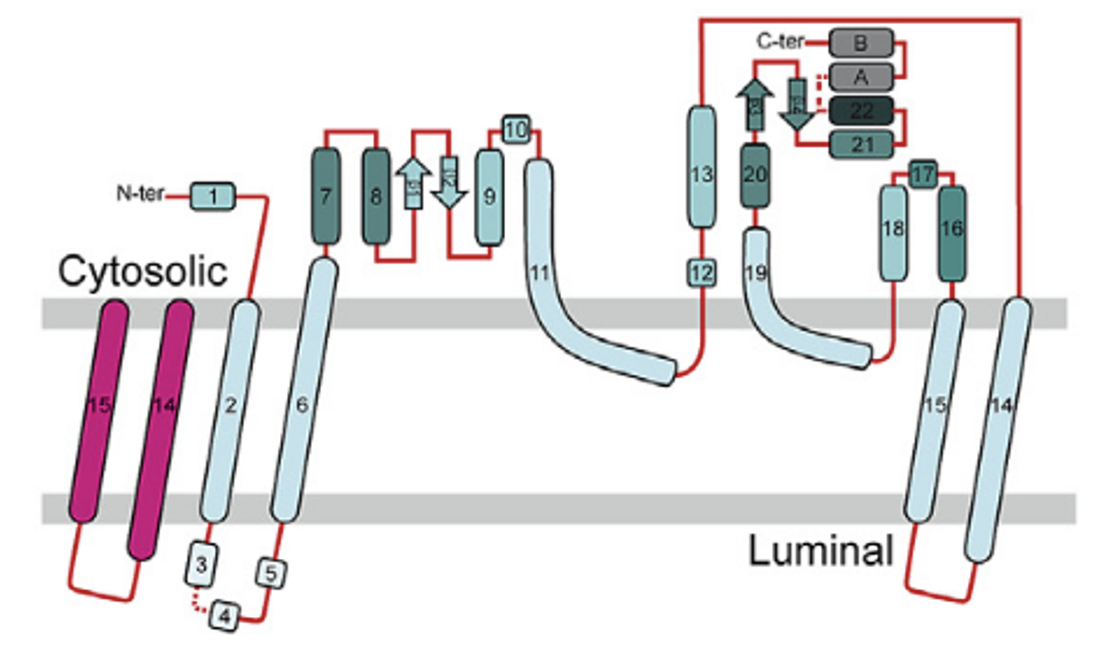
\includegraphics[width=\linewidth]{Pfam/atg9_topo.png}
    \caption{Atg9 Topology}
    \label{fig:atg9_top}
    \small
    Atg9 monomer topology adapted from \cite{guardia2020structure}. Red helices are from and adjacent Atg9 forming the interface. 
\end{figure}


The identification of the DedA re-entrant structural motif (re-entrant loop in contact with its proceeding tranmembrane helix) as well as the unusual Atg9 re-entrant loops prompted an investigation into the prevalence of these structures within Pfam \cite{El-Gebali2019} and the human proteome.


%NEED TO INCLUDE https://journals.plos.org/ploscompbiol/article?id=10.1371/journal.pcbi.1009930


\section{Specific Methods}

\subsection{Building the trRosetta Transmembrane Pfam Database}

\subsubsection{Phase 1}
%other\_reg.txt (contains phobius predicted transmembrane regions), pdb\_pfamA\_reg.txt, pfamseq.txt, pfamA.txt and pfamA\_reg\_seed.txt. 

The following  Pfam-A\_v34.0 files were downloaded from Pfam server for local use: other\_reg.txt,  pfamA.txt and pfamA\_reg\_seed.txt. 

A 'transmembrane protein list' was constructed by filtering the 'other\_reg.txt' file to provide a list of 'pfamseq\_acc' numbers for all sequences with at least one transmembrane region predicted by Phobius \cite{kall2007advantages}. Each 'pfamseq\_acc' in the list was cross-referenced with the  'pfamA\_reg\_seed' table to obtain the Pfam accession numbers of all seed sequences possessing at least one Phobius predicted transmembrane region.  The resulting list was then filtered leaving one (random) seed sequence for each Pfam domain. A final round of filtering was performed to remove any sequences that had less than two predicted transmembrane regions within the Pfam doamin boundaries (Figure \ref{fig:flow_1}).

\begin{figure}[th!]
    \centering
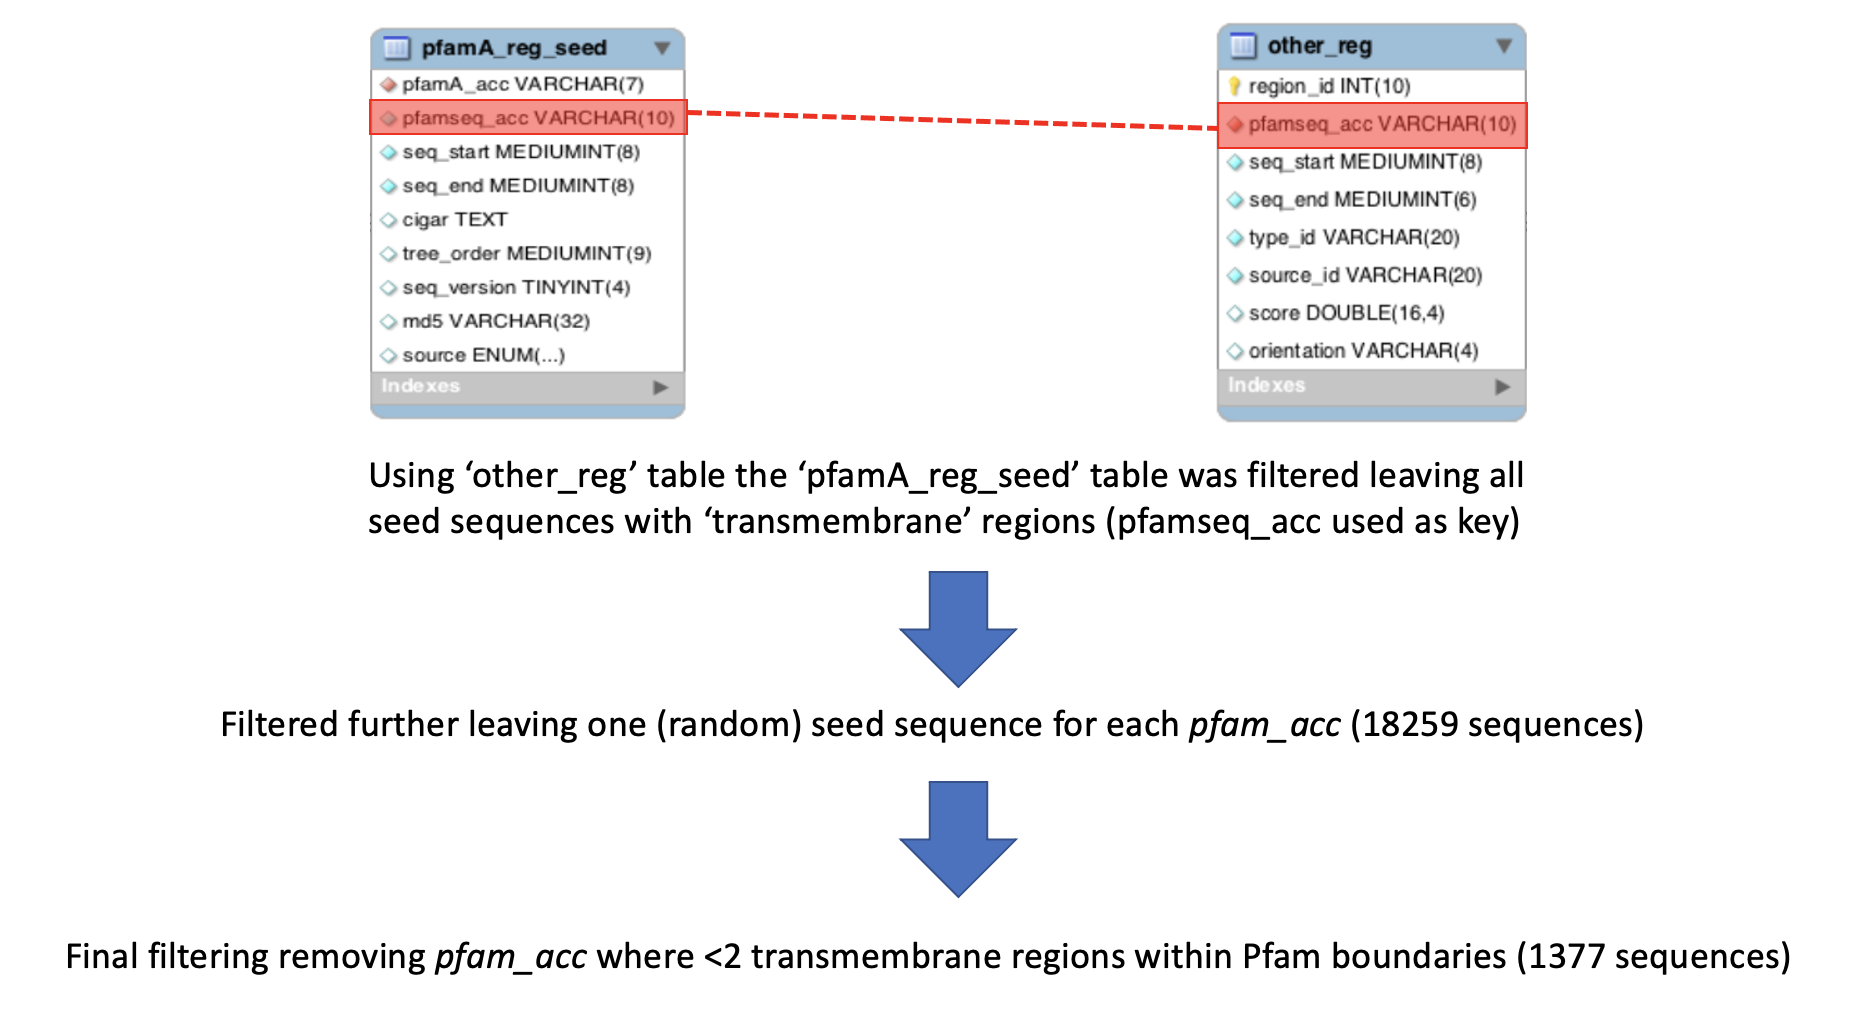
\includegraphics[width=\linewidth]{Pfam/flow_1.png}
    \caption{Pfam transmembrane filtering.}
    \label{fig:flow_1}
    \small
\end{figure}



From a total of 18259 Pfam members, 14538 had no predicted Phobius transmembrane regions; 1401 had at least one transmembrane region outside of the Pfam domain; 944 had one transmembrane region within the Pfam boundaries; 1377 had a minimum of two transmembrane regions with the Pfam boundaries.  The 1337 seed representatives were then modelled using a local installation of trRosetta. 



The models then underwent a local Dali \cite{Holm2016} all against all and the Z-scores were used to cluster the models using CLANS \cite{Frickey2004} with the expectation that clusters resembling Pfam Clans would form. A 0.1 attraction value was used and singletons removed. Examination of the largest cluster revealed not only multiple members of Pfam Clan CL0182 (Ion Transporter Superfamily) but additional Pfam members that were not recorded members of the CL0182 Clan. Investigation into these potentially new members of CL0182 revealed these proteins had multiple Pfam domains resulting in strong structural alignments outside of the Pfam boundaries for the representative Pfam model (Figure \ref{fig:pfam_domain}). 

\begin{figure}[th!]
    \centering
    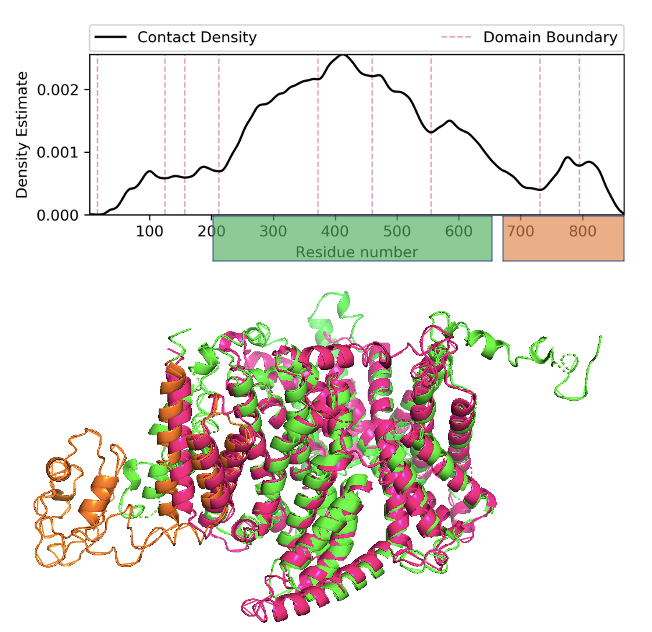
\includegraphics[width=150mm, scale=0.75]{Pfam/pfam_domains.png}
    \caption{Structural alignment of PF11874 model with model of CL0182 member PF06808}
    \label{fig:pfam_domain}
    \small
    Top: Contact density profile for trRosetta model PF11874  with estimated positions of structural domain boundaries.  Green represents CL0182 region. Orange represents PF11874 region. 
    Bottom: Structural alignment of PF11874 trRosetta model with PF06808.  Green represents CL0182 region. Orange represents PF11874 region.  Magenta is the additional Pfam domain.
\end{figure}

In order to overcome this issue the clustering of the models was re-implemented.

\subsubsection{Phase 2}
Models that had only one Pfam domain annotation formed an initial library of 1076 entries. Each of the 261 models that possessed more than one Pfam label were were partitioned into their structural domains using SWORD (Swift and Optimized Recognition of Domains) \cite{postic2017ambiguity} rather than relying on Pfam domain boundaries as these have been shown sometimes not to reflect the actual structural boundaries \cite{mesdaghi2020silico}.  The SWORD output lists a number of partitioning solutions; the highest ranking solution that possessed the whole Pfam domain in one partition was chosen.  This partition was then added to the library. SWORD was unable to partition 25 of the 261 proteins that possessed more than one Pfam domain, in which case the Pfam domain boundaries were used to truncate the model (Figure \ref{fig:sword}).

\begin{figure}[th!]
    \centering
    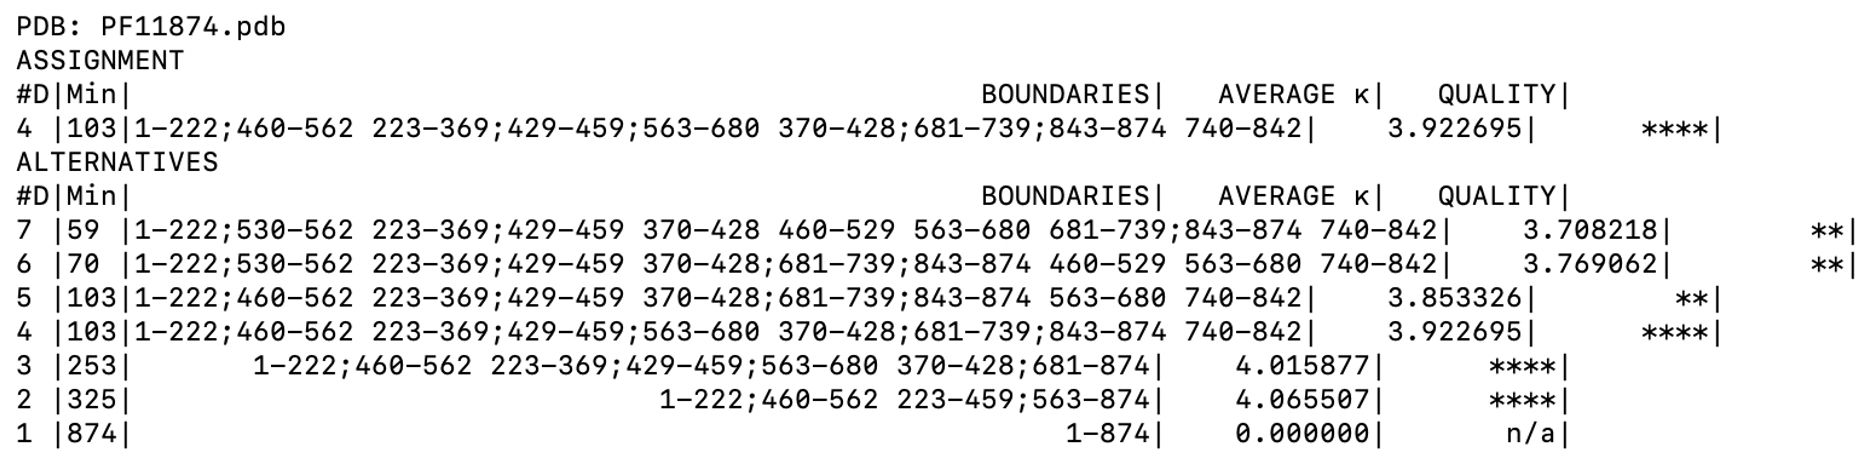
\includegraphics[width=150mm, scale=0.75]{Pfam/sword.png}
    \caption{SWORD output for model PF11874}
    \label{fig:sword}
    \small
\end{figure}

Next, in order to provide validity to the trRosetta modelling of the Pfam domains, available experimental structures were also added to the library. Of the 1337 transmembrane Pfam domains modelled, 306 had at least one experimental structure (5215 structures in total).  2385 of these structures possessed only one Pfam domain which represents 187 out of the 306 Pfam domains with an experimental structure.  These 2385 experimental structures were filtered to leave one representative for an individual Pfam domain (highest resolution selected - if there were equal resolutions both were selected, giving opportunity to include alternative conformations); 222 (for 187 transmembrane Pfam domains) experimental structures representing transmembrane Pfam domains were added to the library.

The sequences of the trRosetta models from the library were then used to mine the EBI AlphaFold database for homologues utilising MrParse \cite{simpkin2021exploiting}. 
For a query sequence MrParse identifies and ranks homologues in the EBI AlphaFold database.  Models with the highest H-score (measure of structural quality; percentage of residues with a given plddt score) were selected.  MrParse provided 865 models that were truncated removing either side of the aligned region.  The 865 AlphaFold models identified were used to supplement the library of trRosetta and experimental models. 165 of the AlphaFold models had an experimental representative in the library (Figure \ref{fig:flow2}). 

\begin{figure}[th!]
    \centering
    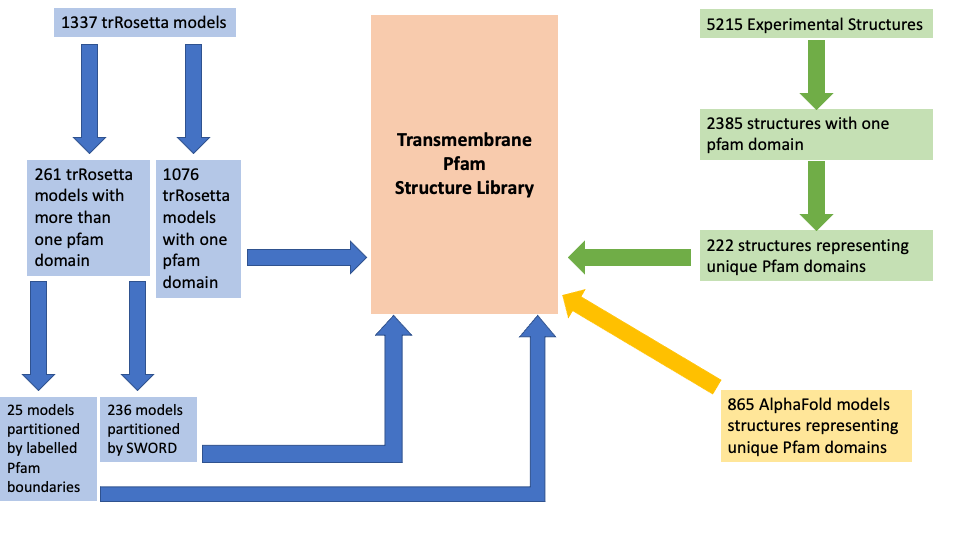
\includegraphics[width=150mm, scale=0.75]{Pfam/flow2.png}
    \caption{Transmembrane Pfam structural library construction}
    \label{fig:flow2}
    \small
\end{figure}



The library then underwent an all-against-all structural alignment using a local installation of Dali.  The Z-scores were then used to cluster the models in CLANS. Initially the default 0.1 attraction value setting with a minimum of one link and singletons were removed. Examination of the largest cluster revealed multiple members of Pfam Clan CL0192 (Rhodopsin Superfamily). In order to determine the optimal attraction value to use in the clustering process, members of the largest cluster were surveyed when clustered using different attraction values. An attraction value of 0.25 was deemed optimal; values above this resulted in loss of Pfam CL0192 members; values below this resulted in additional members of the cluster outside of Pfam CL0192 membership that possessed Z-scores under 5 when aligned with experimental representatives of CL0192.  Also, lowering the attraction value resulted in distribution of Z-scores to ebb towards the lower end (Figure \ref{fig:att_values}).  Utilising the attraction value of 0.25 resulted in the median Z-scores being greater than the mean indicating that the distribution is negatively skewed i.e. the cluster is favouring higher Z-scores.

\begin{figure}[htb]
    \centering % <-- added
\begin{subfigure}{0.4\textwidth}
  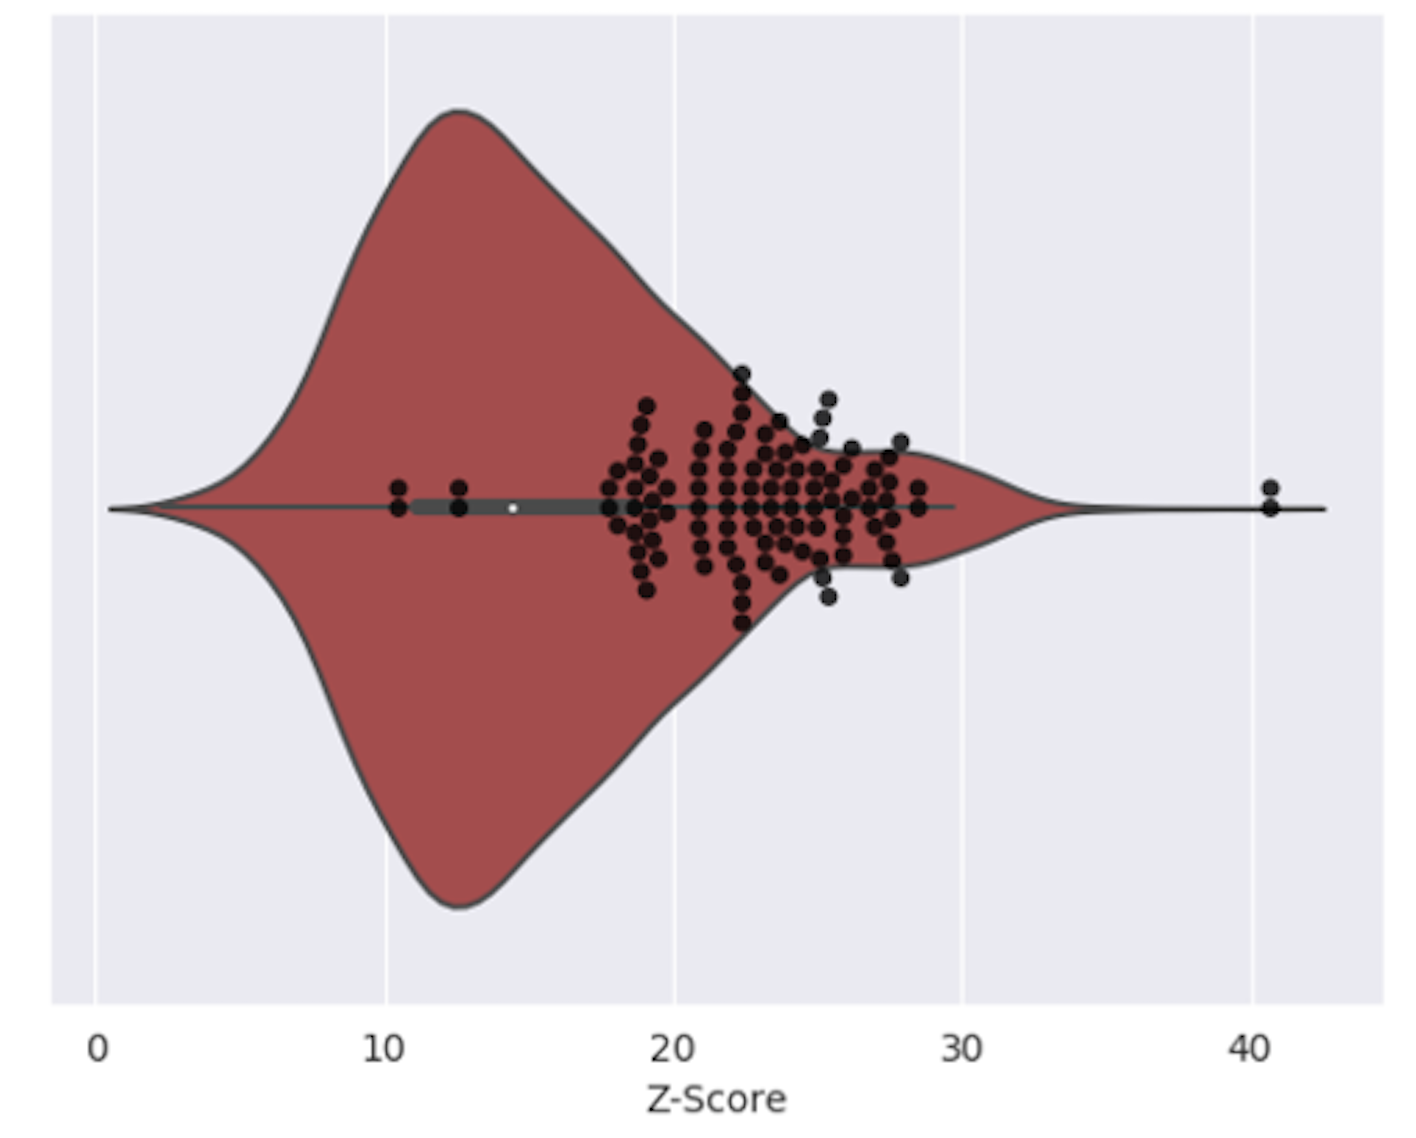
\includegraphics[width=\linewidth]{Pfam/att_val_1.png}
  \caption{Z-score distribution for members of the largest cluster at 0.25 attraction value}
  \label{fig:att1}
\end{subfigure}\hfil % <-- added
\begin{subfigure}{0.4\textwidth}
  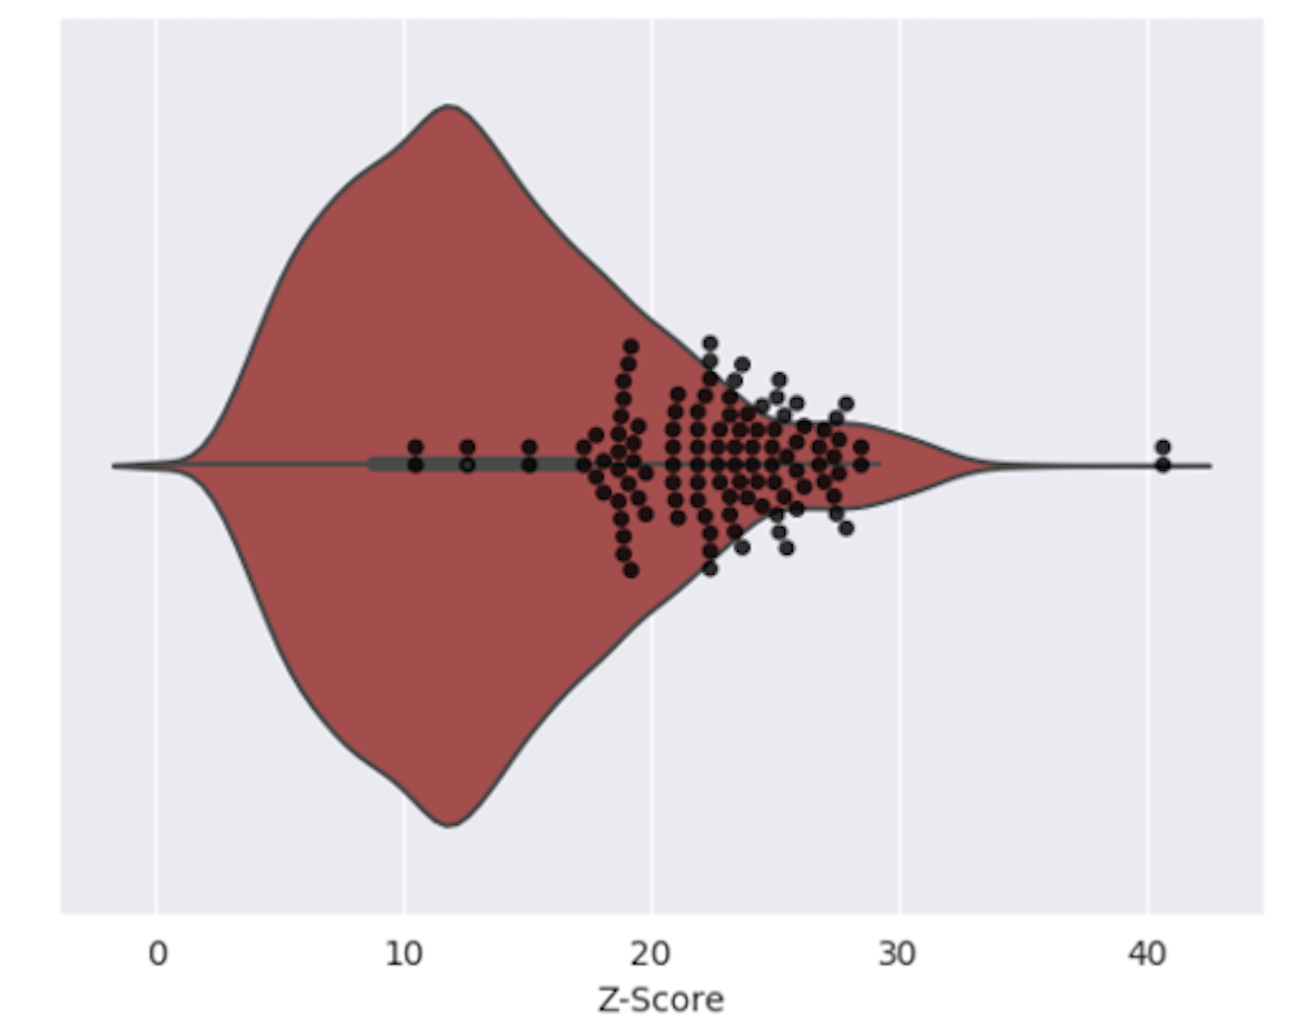
\includegraphics[width=\linewidth]{Pfam/att_val_2.png}
  \caption{Z-score distribution for members of the largest cluster at 0.2 attraction value}
  \label{fig:att2}
\end{subfigure}
\caption{Comparison of Z-score distribution for members of the largest cluster for 0.25 and 0.2 attraction values.}
\small
\begin{flushleft}Violin plots visualising Z-score distribution for the largest cluster.  Superimposed box-plot indicates the range and interquartile range as well median for the Z-scores of the cluster. The superimposed Swarm plot visualised the position within the distribution of Pfam model self-hits (AlphaFold with trRosetta/AlphaFold with experimental/trRosetta with experimental)\end{flushleft}.
\label{fig:att_values}
\end{figure}




\section{Re-entrant loop survey }
A library of re-entrant loop sequences was built by obtaining a non-redundant set of 56 re-entrant helix sequences by first retrieving all 714 TM proteins that contain at least one re-entrant loop from the PDBTM \cite{Kozma2012} and removing redundancy with a 40\% identity threshold. The resulting 127 protein structures were split into their component chains, eliminating any chain lacking a re-entrant loop. As some chains possessed more than one re-entrant loop it resulted in a set of 193 unique re-entrant loop sequences. 

The previous chapters highlighted the presence of proline at the turning points of the re-rentrant loops possessed by the query proteins.  The observation of the presence of proline at this key region of re-entrant loops prompted a survey of the proline content of re-entrant loops. The survey analysed the sequences from the 193 re-entrant loop sequence library and revealed that 44\% (85/193) of structures in the library contained at least one proline residue.  This proportion jumps to 76\% (29/38) when a filter of a minimum re-entant loop length of 18  is applied. This is in contrast to transmembrane helices and interfacial helices (whose sequences were extracted from the PDBTM) where only 39\% (2386/6056) and 30\% (215/712) respectively contain at least one proline residue. Proline is an atypical amino acid as its side chain is connected to the protein backbone twice which results in a five-membered nitrogen-containing ring making it unable to form many of the main chain conformations that can be adopted by the other amino acids \cite{woolfson1990influence};  consequently proline is often located in tight turns where there is sharp change in direction. The presence of proline can also cause kinks in alpha helices as it cannot form a normal helical conformation. Furthermore, there is evidence that even for non-proline kinks, it is proline that first introduced this conformation but subsequently became redundant as tertiary contacts consolidated the structure \cite{yohannan2004evolution}.
Functionally, prolines also prevent membrane protein misfolding \cite{wigley2002protein}.  Interestingly, there are examples where the presence of proline in a re-entrant loop allows it to act as a pivot, enabling the two segments of the loop to switch between states through a conformational change \cite{Kumeta2018,Williamson2015}. Even though the importance of prolines is well understood and transmembrane sequences from the Human Gene Mutation Database \cite{stenson2003human} have one of the highest phenotypic incidences for proline substitutions, their evolution is poorly understood as proline substitutions are difficult establish resulting from the dramatic structural changes that would occur  \cite{partridge2004missense}.  Additionally it has been shown that proline contributes to structural and thermodynamic transmembrane complex stabilization \cite{schmidt2016structural}.  


\section{Pfam Re-entrant Screen}
To screen Pfam for structures that possess the re-entrant/TM helix structural motif, a library of transmembrane Pfam models was constructed (see 5.2.1).  The library contained a trRosetta representative model for each of the 1377 transmembrane Pfam families in addition to being supplemented by 222 experimental structures and 865 AlphaFold models.  The library underwent an all-against-all structural alignment using a local installation of Dali.  164 of the transmembrane Pfam entries in addition to the trRosetta model had a AlphaFold and experimental representative.  As expected, the comparison of the structural alignments of the AlphaFold and trRosetta models with their corresponding experimental structure yielded mean Z-scores of 19.5 with a range of 0.1-60 and 15 with a range of 0.1-40 respectively (Figure \ref{fig:comparison1}). 

\begin{figure}[th!]
    \centering
    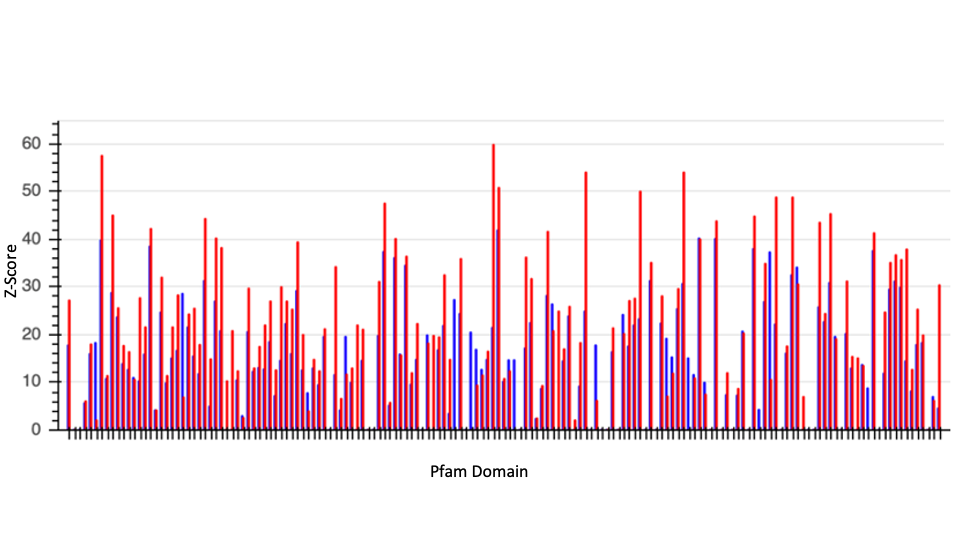
\includegraphics[width=150mm, scale=0.75]{Pfam/tr_af_comp.png}
    \caption{Comparison of trRosetta and AlphaFold2.}
    \label{fig:comparison1}
    \small
    \begin{flushleft}Comparison of the trRosetta and AlphaFold2 structural alignments with their corresponding experimental structure. Red: AlphaFold2; Blue:  trRosetta.\end{flushleft}
\end{figure}

Next the distribution of the Dali Z-scores with their corresponding experimental structure was examined (Figure \ref{fig:comparison2}). For both AlphaFold and trRosetta the modal class Z-score was 10-15 with AlphaFold2 being able to achieve Z-scores beyond 45, outperforming trRosetta.

\begin{figure}[th!]
    \centering
    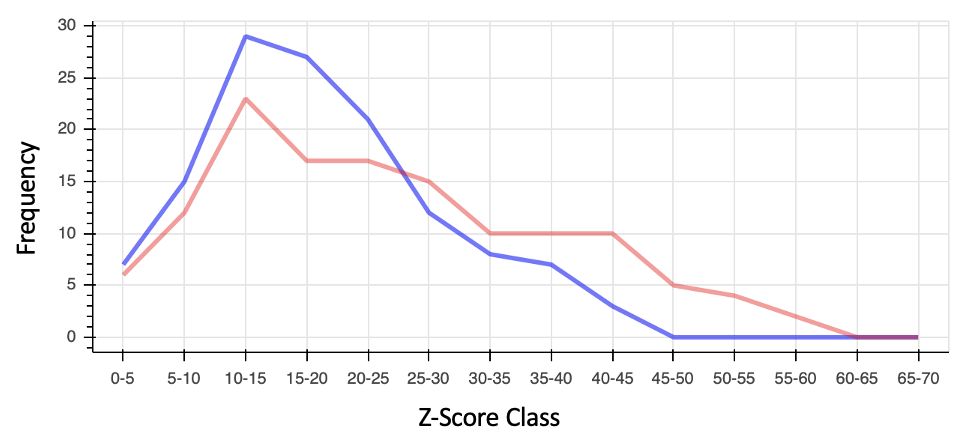
\includegraphics[width=150mm, scale=0.75]{Pfam/comp2.png}
    \caption{Comparison of trRosetta and AlphaFold Structural alignment distributions}
    \label{fig:comparison2}
    \small
    \begin{flushleft}Comparison of the distribution of the trRosetta and AlphaFold structural alignment Dali Z-scores with their corresponding experimental structure. Red: AlphaFold2; Blue: trRosetta.\end{flushleft}
\end{figure}



The Z-scores were then used to cluster the models using CLANS with the expectation that clusters resembling Pfam Clans would form. A 0.25 attraction value was used with a minimum of one link and singletons removed. 

Examination of the largest cluster revealed not only multiple members of Pfam Clan CL0192 (Rhodopsin Superfamily) but additional Pfam members that were not recorded members of the CL0192 Clan. The cluster consisted of a total of 100 members, capturing 39 out of the 45 Pfam representatives of CL0192 members (78 structures in total - trRosetta/AlphaFold/experimental) as well as one out of the CL0347 (Tetraspannin-like) members.  Additionally 11 Pfam representatives (totalling 21) were present that did not belong to a Pfam Clan. Table \ref{table:clustering} gives a breakdown for the 20 largest clusters. Distributions of Z-scores for the 17 largest clusters that possess Pfam domains outside of the dominant Pfam clan are shown in Figure \ref{fig:clusters}   


\begin{table}[]
\caption{Cluster composition of the 20 largest clusters (based on Z-score) of the model library entries}
\begin{tabular}{ccccc}
\rowcolor[HTML]{BFBFBF} 
Cluster & Size & Dominant Clan                                                                & Other Clans  & Possible New Members \\
\rowcolor[HTML]{E9EBF5} 
1       & 100  & CL0192 (39/45)                                                               & CL0347 (1/6) & 11                   \\
2       & 47   & CL0015 (20/23)                                                               & N/A          & 3                    \\
\rowcolor[HTML]{E9EBF5} 
3       & 37   & CL0062 (15/20)                                                               & N/A          & 1                    \\
4       & 32   & CL0182 (19/19)                                                               & N/A          & 3                    \\
\rowcolor[HTML]{E9EBF5} 
5       & 30   & CL0111 (16/19)                                                               & N/A          & 5                    \\
6       & 27   & CL0064 (12/13)                                                               & CL0142 (1/7) & 1                    \\
\rowcolor[HTML]{E9EBF5} 
7       & 25   & CL0184 (13/22)                                                               & N/A          & 0                    \\
8       & 19   & CL0375 (8/13)                                                                & CL0396 (1/2) & 2                    \\
\rowcolor[HTML]{E9EBF5} 
9       & 14   & \multicolumn{1}{l}{\cellcolor[HTML]{E9EBF5}All exp struct from 6 Pfam clans} & N/A          & N/A                  \\
10      & 13   & CL0222 (5/7)                                                                 & N/A          & 1                    \\
\rowcolor[HTML]{E9EBF5} 
11      & 12   & CL0181 (8/17)                                                                & N/A          & 1                    \\
12      & 12   & CL0308 (3/3)                                                                 & CL0340 (2/4) & 3                    \\
\rowcolor[HTML]{E9EBF5} 
13      & 11   & CL0062 (5/20)                                                                & N/A          & 1                    \\
14      & 11   & CL0176 (4/4)                                                                 & N/A          & 1                    \\
\rowcolor[HTML]{E9EBF5} 
15      & 11   & CL0315 (10/11)                                                               & N/A          & 0                    \\
16      & 10   & CL0322 (5/5)                                                                 & N/A          & 0                    \\
\rowcolor[HTML]{E9EBF5} 
17      & 8    & CL0307 (6/9)                                                                 & N/A          & 0                    \\
18      & 8    & N/A                                                                          & N/A          & 5                    \\
\rowcolor[HTML]{E9EBF5} 
19      & 8    & CL0425 (2/3)                                                                 & N/A          & 2                    \\
20      & 7    & N/A                                                                          & N/A          & 3                   
\end{tabular}
\small
Values in the size column represent the total number of models in the cluster. Values in parenthesis indicate the number of unique Pfam model accessions out of total established members present in the cluster.  Values in the possible new members column are the number of unique Pfam model accessions present in the cluster that do not belong to the dominant clan.
\label{table:clustering}
\end{table}




 \begin{figure}[htb]
    
    \centering % <-- added
\begin{subfigure}{0.2\textwidth}
  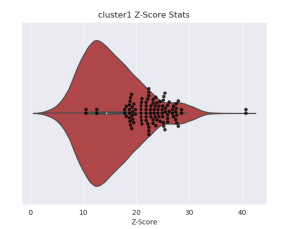
\includegraphics[width=\linewidth]{Pfam/cl01.png}
  \caption{Cluster 1}
  \label{fig:cl01}
\end{subfigure}\hfil % <-- added
\begin{subfigure}{0.2\textwidth}
  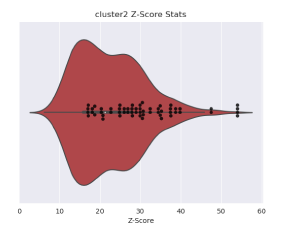
\includegraphics[width=\linewidth]{Pfam/cl02.png}
  \caption{Cluster 2}
  \label{fig:cl02}
\end{subfigure}\hfil % <-- added
\begin{subfigure}{0.2\textwidth}
  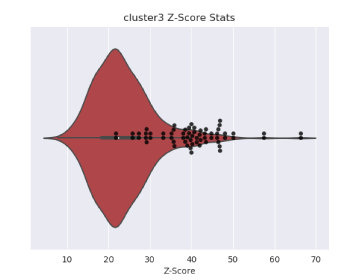
\includegraphics[width=\linewidth]{Pfam/cl03.png}
  \caption{Cluster 3}
  \label{fig:cl03}
\end{subfigure}\hfil % <-- added
\begin{subfigure}{0.2\textwidth}
  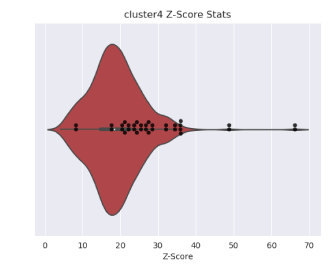
\includegraphics[width=\linewidth]{Pfam/cl04.png}
  \caption{Cluster 4}
  \label{fig:cl04}
\end{subfigure}\hfil % <-- added
\begin{subfigure}{0.2\textwidth}
  
  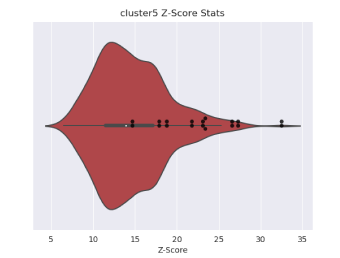
\includegraphics[width=\linewidth]{Pfam/cl05.png}
  \caption{Cluster 5}
  \label{fig:cl05}
\end{subfigure}\hfil % <-- added
\begin{subfigure}{0.2\textwidth}
  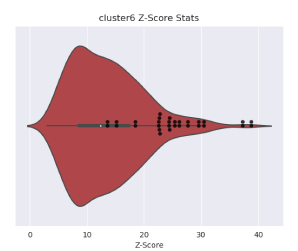
\includegraphics[width=\linewidth]{Pfam/cl06.png}
  \caption{Cluster 6}
  \label{fig:cl06}
\end{subfigure}\hfil % <-- added
\begin{subfigure}{0.2\textwidth}
  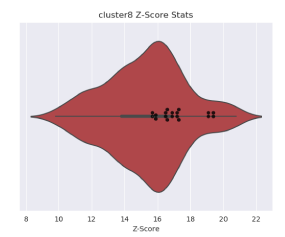
\includegraphics[width=\linewidth]{Pfam/cl08.png}
  \caption{Cluster 8}
  \label{fig:cl08}
\end{subfigure}\hfil % <-- added
\begin{subfigure}{0.2\textwidth}
  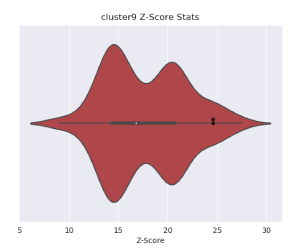
\includegraphics[width=\linewidth]{Pfam/cl09.png}
  \caption{Cluster 9}
  \label{fig:cl09}
\end{subfigure}\hfil % <-- added
\begin{subfigure}{0.2\textwidth}
  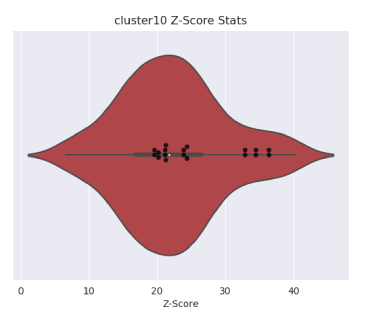
\includegraphics[width=\linewidth]{Pfam/cl10.png}
  \caption{Cluster 10}
  \label{fig:cl10}
\end{subfigure}\hfil % <-- added
\begin{subfigure}{0.2\textwidth}
  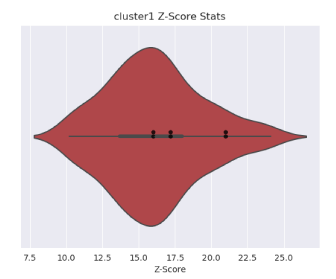
\includegraphics[width=\linewidth]{Pfam/cl11.png}
  \caption{Cluster 11}
  \label{fig:cl11}
\end{subfigure}\hfil % <-- added
\begin{subfigure}{0.2\textwidth}
  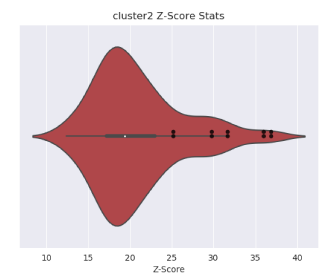
\includegraphics[width=\linewidth]{Pfam/cl12.png}
  \caption{Cluster 12}
  \label{fig:cl12}
\end{subfigure}\hfil % <-- added
\begin{subfigure}{0.2\textwidth}
  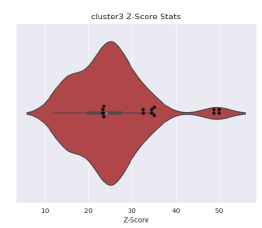
\includegraphics[width=\linewidth]{Pfam/cl13.png}
  \caption{Cluster 13}
  \label{fig:cl13}
\end{subfigure}\hfil % <-- added
\begin{subfigure}{0.2\textwidth}
  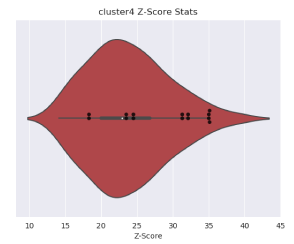
\includegraphics[width=\linewidth]{Pfam/cl14.png}
  \caption{Cluster 14}
  \label{fig:cl14}
\end{subfigure}\hfil % <-- added
\begin{subfigure}{0.2\textwidth}
  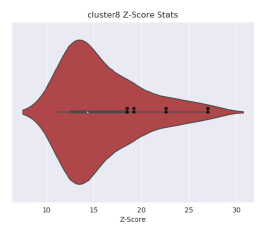
\includegraphics[width=\linewidth]{Pfam/cl18.png}
  \caption{Cluster 18}
  \label{fig:cl18}
\end{subfigure}\hfil % <-- added
\begin{subfigure}{0.2\textwidth}
  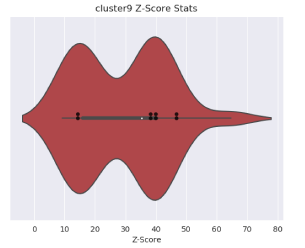
\includegraphics[width=\linewidth]{Pfam/cl19.png}
  \caption{Cluster 19}
  \label{fig:cl19}
\end{subfigure}\hfil % <-- added
\begin{subfigure}{0.2\textwidth}
  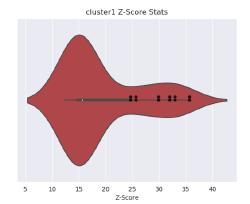
\includegraphics[width=\linewidth]{Pfam/cl20.png}
  \caption{Cluster 20}
  \label{fig:cl20}
\end{subfigure}\hfil % <-- added

\caption{Z-score distribution visualisations for the 16 largest clusters possessing Pfam domains outside of the dominant Pfam clan}
\small
\begin{flushleft}Violin plots: Z-score distribution. Box-plots: range/interquartile range/median. Swarm plot: position within the distribution of Pfam model self-hits (AlphaFold with trRosetta/AlphaFold with experimental/trRosetta with experimental) \end{flushleft}.
\label{fig:clusters}
\end{figure}

Cluster 9 was made up of experimental structures spanning 6 different Pfam families.  Visual inspection of the structural alignments showed that the structurally diverse transmembrane regions possessed beta sheet architecture in common.  Analysis with HHpred against these beta sheet regions  to detect homologous domains showed that they were Ig-like domains.

Surveying the members of cluster 1, 6, 8, and 12 revealed that members of two Pfam clans were present in addition to Pfam representatives not belonging to any clan.  For example, cluster 8 consisted of 19 members; 16 (8 unique Pfam members) belonged to CL0375 (Transporter superfamily, four TM region of clan 13 members); 1 member (PF01284) belonged to CL0396 (The MAL and related proteins for vesicle trafficking and membrane link (MARVEL) domain of 2 clan members); 2 (PF15108 and PF14985) did not belong to any Pfam clan.  Visual inspection of the structural alignments between the crystal representative of CL0375 (PF00822 - pdb code: 4P79), the CL0396 members and the Pfam models not belonging to a clan  show strong simularity that is indicative of homology (Figure \ref{fig:cluster_8}).

\begin{figure}[th!]
    \centering
    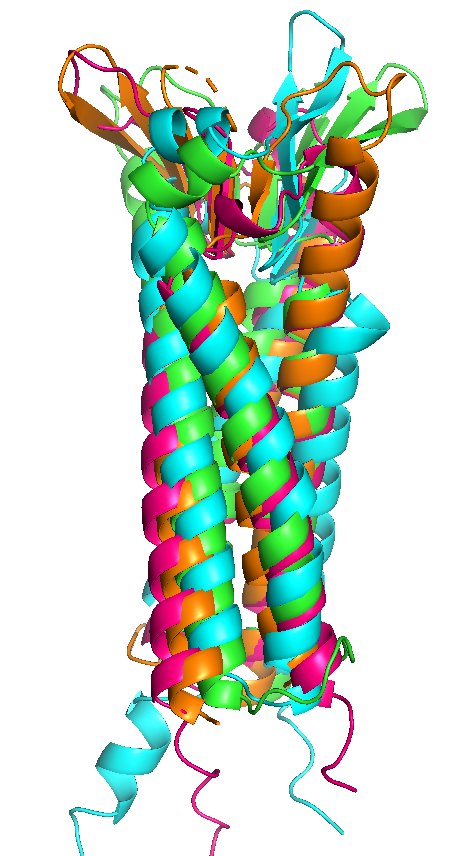
\includegraphics[width=75mm, scale=0.75]{Pfam/cluster_8.png}
    \caption{Structural alignment for Cluster 8 members}
    \label{fig:cluster_8}
    \small
    \begin{flushleft}Dali structural alignment for CL0375 member PF00822 - pdb code: 4P79 (green); CL0396 member, PF01284 (AF2 model) (magenta); PF15108 (AF2 model) (Orange); PF14985 (AF2 model)(cyan). \end{flushleft}
\end{figure}

Both PF15108 and PF14985 do not currently belong to any Pfam clan. PF14985 (TMEM140) has been shown to suppress the viability, migration, and invasion of cancer cells \cite{refaat2018retrospective}.  A HHpred screen of a PF14985 representative against Pfam show a 100\% probability hit with PF15108 (as well as itself).  PF15108, also known as TMEM37, is a voltage-dependent calcium channel gamma-like subunit protein. The $\gamma$ subunits are a family of 8 protein subunits; type 1,6 are regulators for trafficking & activation of muscle voltage dependent calcium channel (VDCC); types 2,3,4,8 are involved in the AMPA glutamate receptor localisation in the brain; type 5 and 7 have an unknown function \cite{chen2007calcium}.

Two of the clusters (18 and 20) contained Pfam families that were not labelled as Pfam clans.  Cluster 18 was composed of 5 bacterial DUFs (PF06790, PF04854, PF06161,PF07264, PF09955).    Cluster 20 was made up of 3 unique Pfam representatives (PF00230, PF10136, PF01226) across 7 models. PF01226 (Major intrinsic protein\_MIP) and PF01226 (Formate/nitrite transporter) are both transporters, however, PF10136 is labelled as 'Site-specific recombinase'. The structural alignment of the trRosetta model of PF10136 from cluster 20 with an experimental structure representative (PF01226, 3TDS) from the cluster (Figure \ref{fig:PF10136}) shows obvious structural homology.  This structural match contradicted   its Pfam annotated functions.  Indeed, during  this investigation Pfam was updated and the new version included a new Clan linking PF00230, PF10136 and PF01226 together (CL0716 - Aquaporin-like).  Additionally further annotation for the PF10136 entry states that there is no evidence that PF10136 is a recombinase and this may be a misannotation.

\begin{figure}[th!]
    \centering
    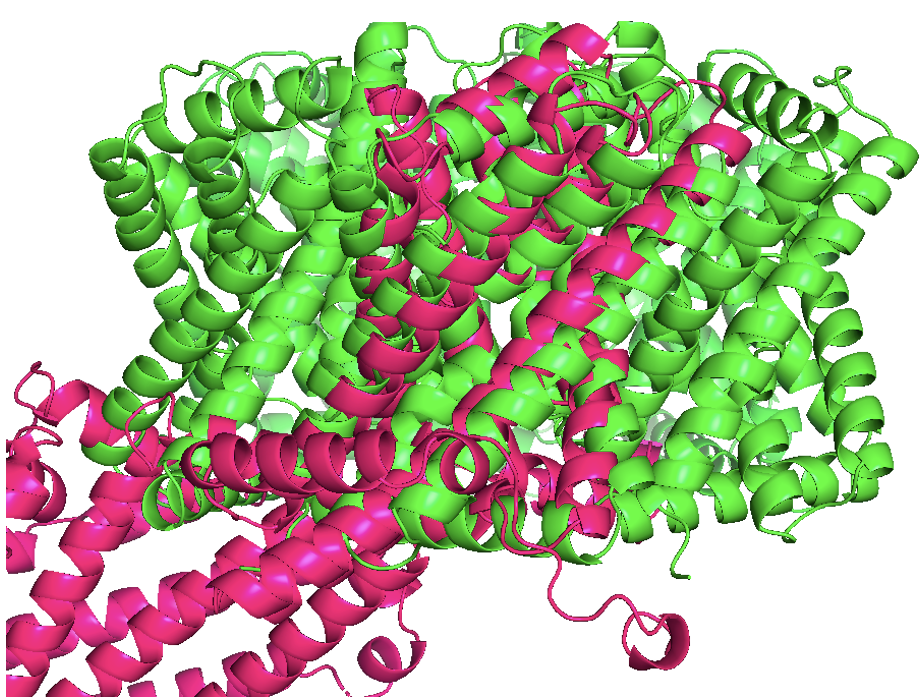
\includegraphics[width=75mm, scale=0.75]{Pfam/PF10136.png}
    \caption{Structural alignment between PF10136 and 3DTS}
    \label{fig:PF10136}
    \small
    Dali structural alignment for PF10136 (magenta) and 3DTS (green)
\end{figure}

In summary, the clustering of the transmembrane Pfam model library identified homology beyond what sequence analysis can accomplish.  The clustering was successful in identifying new homology connections between Pfam members such as the PF15108 and PF14985 being structural neighbours to members of the CL0375 Pfam clan.  The exercise also showed links between Pfam members that did not currently belong to a Pfam clan;  PF00230, PF10136 and PF01226.  Furthermore, the clustering exercise identified links between clans that were not previously known; CL0375 and CL0396.  


\subsection{Pfam Re-entrant/TM helix structural motif Screen}

Figure \ref{fig:rent_loop} shows the Re-entrant/TM helix structural motif motif (re-entrant loop in contact with its proceeding tranmembrane helix) that was identified during the investigation into the structure and function of the DedA protein family.  These motifs have only been reported in tranporter proteins.  The identification of the DedA re-entrant structural motif prompted an investigation into the prevalence of these structures within Pfam \cite{El-Gebali2019} as well as to being able to infer transporter function for Pfam families that have an unknown function.

\begin{figure}[th!]
    \centering
    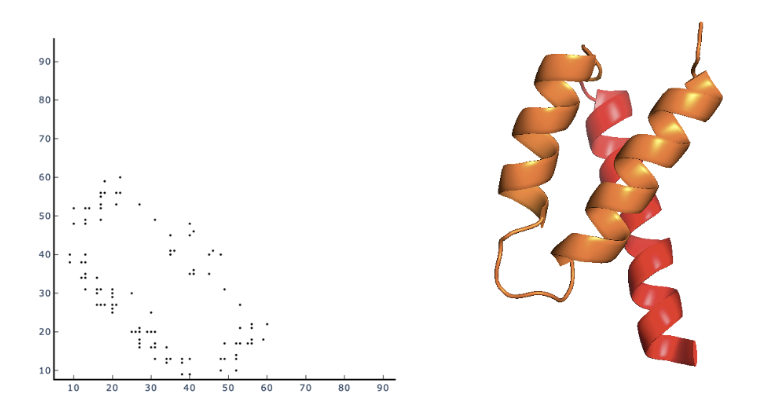
\includegraphics[width=100mm, scale=0.99]{Pfam/rent_loop.png}
    \caption{Re-entrant/TM helix motif}
    \label{fig:rent_loop}
    \small
    \begin{flushleft}
Left: Re-entrant/TM helix motif contact map. Right: strutural model of Re-entrant/TM helix motif (red: transmembrane helix, orange: re-entrant loop).\end{flushleft}

\end{figure}

The re-entrant/TM helix structural motif library of 192 members (see Chapter 3 methods) underwent a pairwise screen against the Pfam transmembrane library using a local installation of Dali.

An initial check looked at the hits for the N-terminal re-entrant/TM helix structural motif from the eukaryotic CLC transporter 3ORG \cite{Feng2010}.  As expected the top hit with a Z-score of 6.1 was with the PF00654 (CLC transporter family) (Figure \ref{fig:clc}).

\begin{figure}[th!]
    \centering
    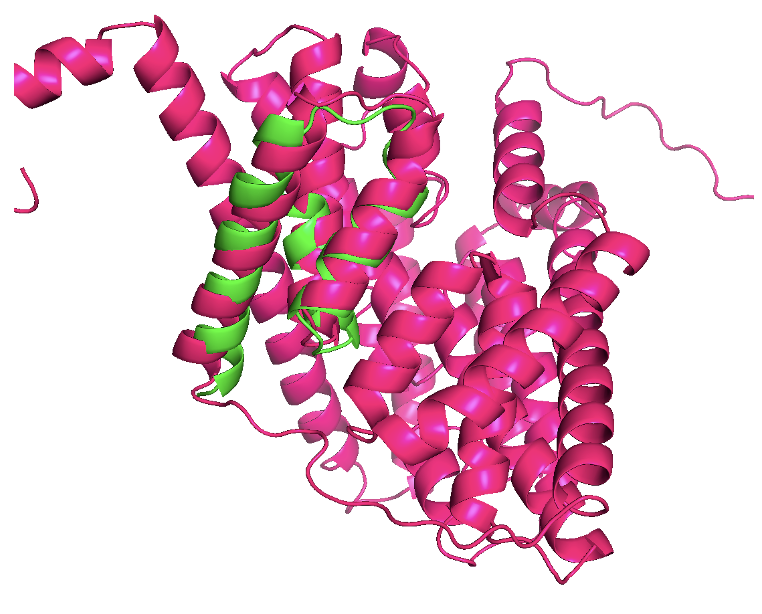
\includegraphics[width=75mm, scale=0.75]{Pfam/clc.png}
    \caption{Structural alignment between PF00654 (CLC) and 3ORG re-entrant/TM helix structural motif}
    \label{fig:clc}
    \small
   \begin{flushleft}
 Dali structural alignment for PF00654 (CLC) (magenta) and 3ORG N-terminal re-entrant/TM helix structural motif (green).\end{flushleft}

\end{figure}

Additionally, as expected, inspection of the re-entrant/TM helix structural motif hits for PF09335 (SNARE\_assoc - DedA domain) (Figure \ref{fig:tmem}) and PF06695 (Sm\_multidrug\_ex - member of the DedA superfamily) (Figure \ref{fig:sm}) brought together the re-entrant/TM helix structural motif of 3ORG, 5TQQ, 3ND0, 3DET, 6COY (all Cl\textsuperscript{-}/H\textsuperscript{+} antiporters), 5l25 (boron exchanger), 2n4x (electron transporter - albeit classified as a member of the lysine exporter superfamily \cite{Saier2016}) and 5z10 (mechanogated channel), all with Z-scores between 4 and 6.1.  


\begin{figure}[htb]
    \centering % <-- added
\begin{subfigure}{0.3\textwidth}
  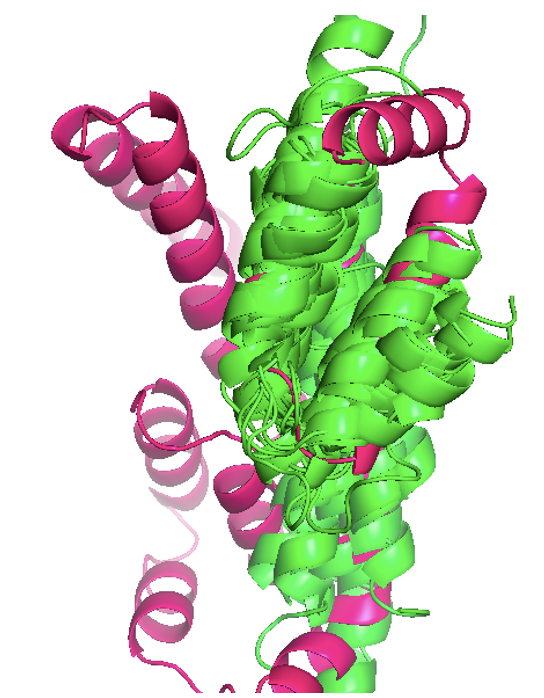
\includegraphics[width=\linewidth]{Pfam/PF09335.png}
  \caption{Re-entrant/TM helix structural motif hits for PF09335 (SNARE\_assoc - DedA domain)}
  \label{fig:tmem}
\end{subfigure}\hfil % <-- added
\begin{subfigure}{0.3\textwidth}
  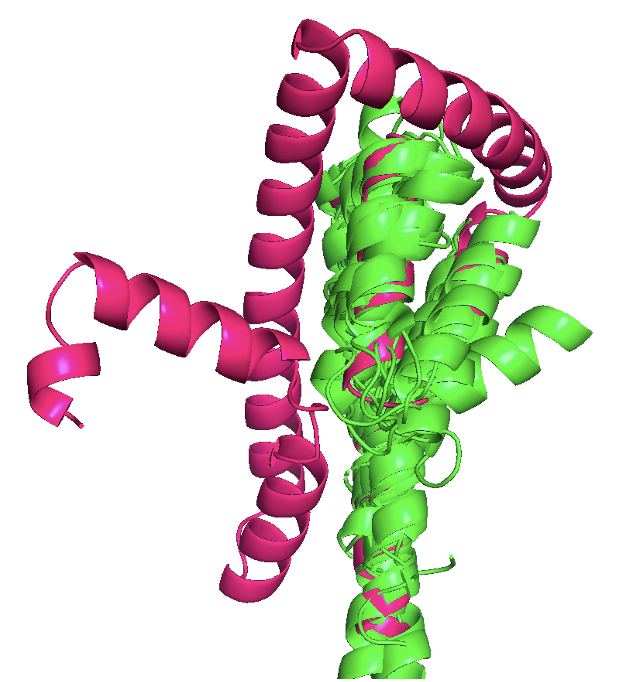
\includegraphics[width=\linewidth]{Pfam/PF06695.png}
  \caption{Re-entrant/TM helix structural motif hits PF06695 (Sm\_multidrug\_ex - member of the DedA super family)}
  \label{fig:sm}
\end{subfigure}
\caption{Re-entrant/TM helix structural motif hits for PF09335 and PF06695}
\small
Magenta - Pfam representative model; Green are the Re-entrant/TM helix structural hits. 
\label{fig:deda}
\end{figure}

Next the Pfam model hits for the re-entrant loop/TM helix  structural motif that had a Z-score greater than 4 were examined (Table \ref{table:3org_hits} ).


\begin{table}[]
\caption{Dali hits for 3org re-entrant loop/TM helix structural motif}
\resizebox{\columnwidth}{!}{%
\begin{tabular}{lllll}
\rowcolor[HTML]{E2EFDA} 
Hit Name & CLAN   & z   & Pfam Name                             & Pfam Description                                                                                                                                                                 \\
\rowcolor[HTML]{FFFFC7} 
PF13194  & NULL   & 5.2 & Domain of unknown function (DUF4010)  & \begin{tabular}[c]{@{}l@{}}This is a family of putative membrane proteins \\ found in archaea and bacteria.    \\ It is sometimes found C terminal to Pfam:PF02308.\end{tabular} \\
\rowcolor[HTML]{FFFC9E} 
PF10852  & NULL   & 4.6 & Protein of unknown function (DUF2651) & \begin{tabular}[c]{@{}l@{}}This family of proteins with unknown function appears \\ to be restricted to Bacillus spp.\end{tabular}                                               \\
\rowcolor[HTML]{FFFFC7} 
PF06450  & CL0182 & 4.4 & Bacterial Na\textsuperscript{+}/H\textsuperscript{+} antiporter B (NhaB)  & \begin{tabular}[c]{@{}l@{}}This family consists of several bacterial Na\textsuperscript{+}/H\textsuperscript{+} antiporter B \\ (NhaB) proteins. The exact function of this family is unknown.\end{tabular}          \\
\rowcolor[HTML]{FFFC9E} 
PF03606  & CL0182 & 4.2 & C4-dicarboxylate anaerobic carrier    & NULL                                                                                                                                                                             \\
\rowcolor[HTML]{FFFFC7} 
PF03806  & CL0182 & 4   & AbgT putative transporter family      & NULL                                                                                                                                                                            
\end{tabular}
}
\label{table:3org_hits}
\end{table}


Three of the hits with the Chloride channel re-entrant loop/TM helix structural motif belong to the Pfam clan CL0182 (Ion Transporter (IT) Superfamily).  Members of this family are known to possess re-entrant loops and have an pseudo inverse repeat topology.  A more detailed examination of this clan is detailed in Chapter 6.  Additionally two other significant hits were recorded; both being bacterial domains of unknown function (PF13194 - DUF4010 and PF10852 - DUF2651).  It can be seen from visual inspection of the structural alignment of the PF10852 model and the 3ORG query motif that DUF2651 does not possess the re-entrant/TM helix motif and was a false positive hit (Figure \ref{fig:10852}).  Inspection of the PF13194 structural alignment (Figure \ref{fig:13194}) verifies that DUF4010 does indeed possess the query motif.


\begin{figure}[htb]
    \centering % <-- added
\begin{subfigure}{0.3\textwidth}
  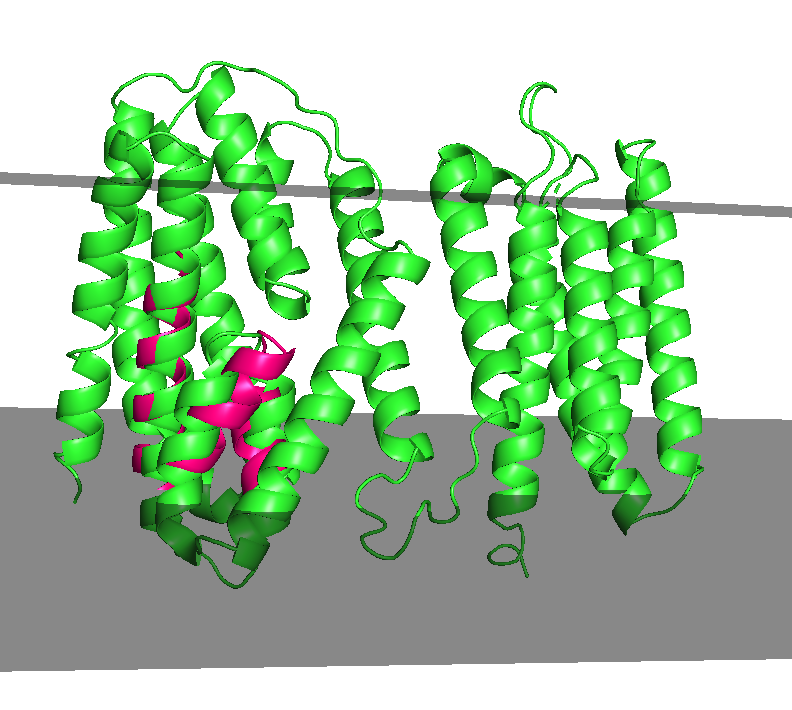
\includegraphics[width=\linewidth]{Pfam/13194.png}
  \caption{Structural alignment of re-entrant/TM helix structural motif of 3ORG with the PF13194 model}
  \label{fig:13194}
\end{subfigure}\hfil % <-- added
\begin{subfigure}{0.3\textwidth}
  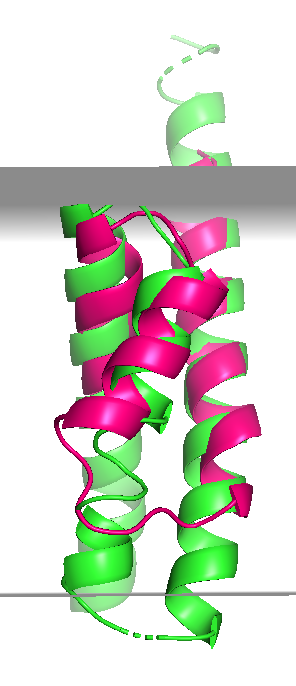
\includegraphics[width=\linewidth]{Pfam/10852.png}
  \caption{Structural alignment of re-entrant/TM helix structural motif of 3org with the PF10852 model}
  \label{fig:10852}
\end{subfigure}
\caption{Re-entrant/TM helix structural motif structural alignments with PF13194 and PF10852}
\small
\begin{flushleft}
Green - Pfam representative model; Magenta are the Re-entrant/TM helix structural motif from 3org. \end{flushleft}

\label{fig:mg_trans}
\end{figure}

A detailed inspection of the representative model of DUF4010 shows two transmembrane domains where the N-terminal domain represents PF02308 and the C-terminal domain represents PF10852.  The PF10852 domain possess two re-entrant/TM helix motifs facing each other in the membrane and contributes to a pseudo inverse repeat architecture that is only known to be found in transporters.  An investigation into common domain organisation structures involving DUF4010 identified that DUF4010 is commonly found with MgtC (PF02308) which also has an unknown function.  MgtC is, however, known to be found in an operon with the Mg\textsuperscript{2+} transporter ATPase protein MgtB \cite{moncrief1999magnesium}.  The observation that PF10852 possesses re-entrant/TM helix motifs facing each other in the membrane and part of a pseudo inverse repeat architecture suggests it is a transporter; the fact that PF10852 is commonly found in proteins with the Pfam domain MgtC which is transcribed along side MgtB suggests that PF10852 is transporting a substrate relating to the transport of Mg\textsuperscript{2+}.


\section{Re-entrant/TM helix motif human AlphaFold database Screen}

The availability of the new highly accurate AlphaFold2 models gave the opportunity to identify the presence of re-entrant/TM helix motifs in other proteins within the human proteome.  The human AlphaFold database \cite{david2022alphafold} was screened with the both the N- and C-terminal re-entrant/TM helix motif from a human, bacterial and archaeal DedA representative; Tmem41b, YqjA and Mt2055, respectively. The screen resulted in a list of 559 non redundant hits with a Z-score of more than 4.  This list was further filtered removing hits that were predicted not to possess a minimum of one transmembrane helix.  The structural alignments of the resulting 217 hits were visually inspected for the presence of re-entrant loops (Figure \ref{fig:hits}).

\begin{figure}[htb]
    \centering % <-- added
\begin{subfigure}{0.3\textwidth}
  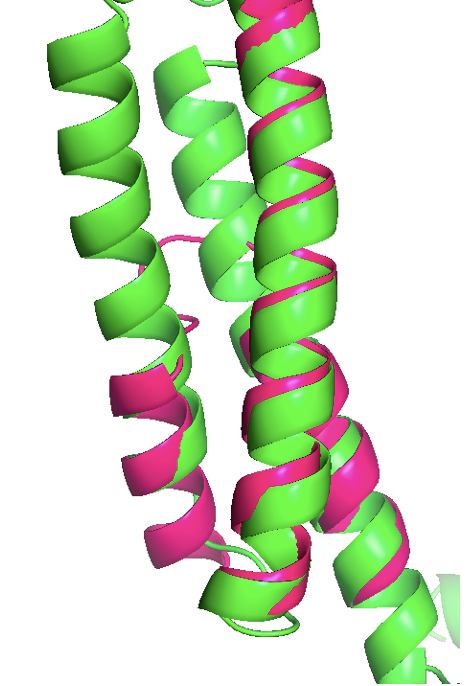
\includegraphics[width=\linewidth]{Pfam/slc2.png}
  \caption{Mt2055 C-terminal re-entrant/TM helix motif (magenta) structural alignments with the AlphaFold2 Solute Carrier Family 2 Facilitated Glucose Transporter (green)}
  \label{fig:false_pos}
\end{subfigure}\hfil % <-- added
\begin{subfigure}{0.3\textwidth}
  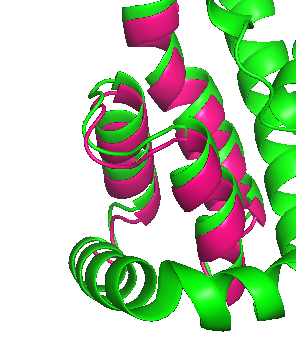
\includegraphics[width=\linewidth]{Pfam/tmb_w_tmb.png}
  \caption{Self-hit of Tmem41b C-terminal re-entrant motif (magenta) structural alignments with the Tmem41b C-terminal re-entrant motif (green)}
  \label{fig:self_hit}
\end{subfigure}
\caption{False positive hits. }
\small
False positive hits were mainly due to the re-entrant loop of the query structure aligning with two transmembrane helices in contact with one another (a) as opposed to a true positive hit where the query clearly has aligned with a corresponding re-entrant/TM helix structural motif (b)
\label{fig:hits}
\end{figure}

Thirty proteins were determined to exhibit a re-entrant loop/TM helix motif within the structurally aligned region.  The OMP server was then used to place the structures into a plasma membrane in order to determine whether the re-entrant motif actually sits within the membrane bi-layer boundaries rather than being part of a globular domain.  Indeed, performing a re-entrant/TM helix motif screen against the full PDB using PDBeFold \cite{krissinel2004secondary} it can be seen that these structural motifs are also found in globular proteins e.g. 4xrm (Figure \ref{fig:4xa}).  Furthermore examination of the hydrophobicity profile of the globular equivalent re-entrant/TM helix motif reveals the same inconsistent hydrophobicity distribution as seen in tranmembrane re-entrant loops where C terminal side is more hydrophilic (figure \ref{fig:4xb}).

\begin{figure}[htb]
    \centering % <-- added
\begin{subfigure}{0.3\textwidth}
  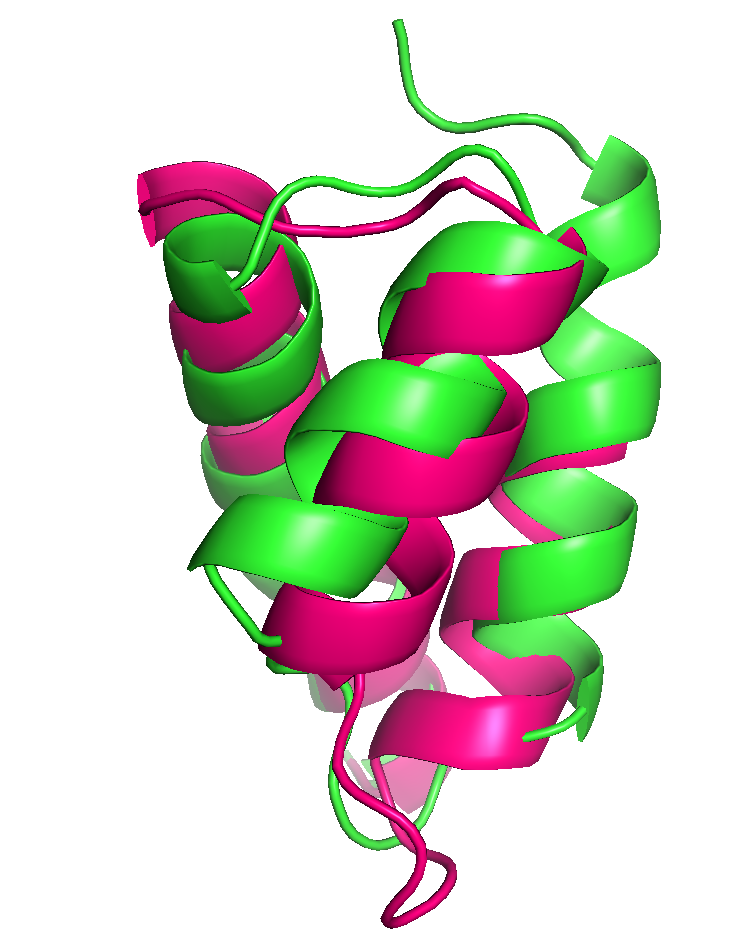
\includegraphics[width=\linewidth]{Results/4x_6c_super.png}
  \caption{4xrm (green) superposition with 6cb2 (magenta) re-entrant/TM helix motif}
  \label{fig:4xa}
\end{subfigure}\hfil % <-- added
\begin{subfigure}{0.3\textwidth}
  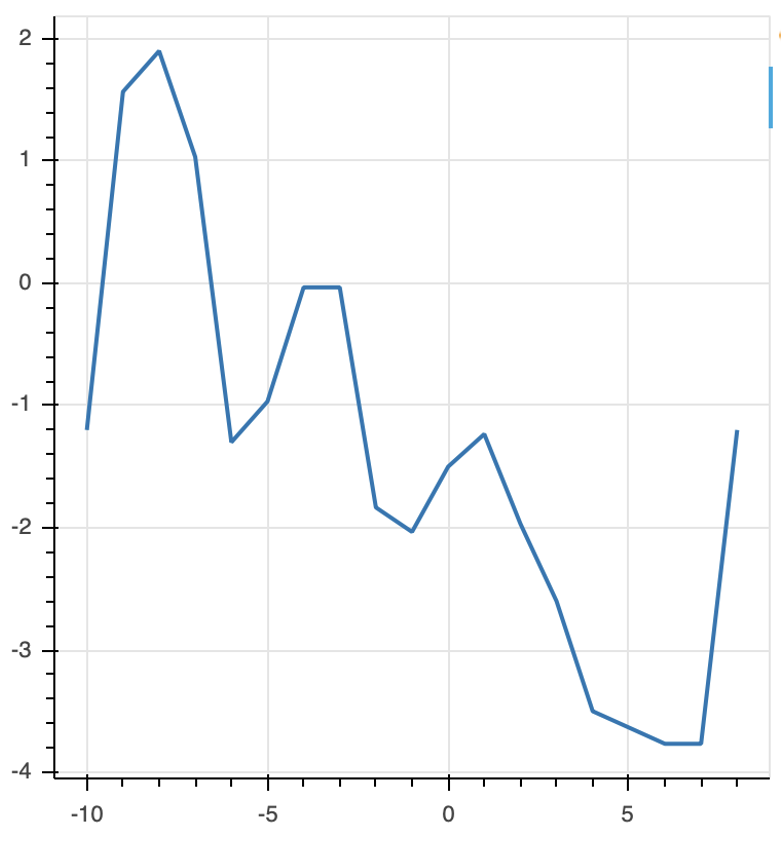
\includegraphics[width=\linewidth]{Results/4x_hydro.png}
  \caption{4xrm hydrophobicity distribution. (abscissa:residue position, ordinate: smoothed hydrophobicity)}
  \label{fig:4xb}
\end{subfigure}
\caption{4xrm comparison with 6cb2 re-entrant/TM helix structural motif }
\small
\label{fig:4x}
\end{figure}


Subsequently, 27 of the 30 models were confirmed to possess the re-entrant loop/TM helix motif within the membrane boundaries after visual inspection (see example Figure \ref{fig:q6q}).  Furthermore, the detailed visual inspection revealed that in 16 of the models although the re-entrant loop/TM helix motif was positioned within the membrane bi-layer, the helices of the re-entrant loop were atypically long with 5-6 helical turns on the N- and C- terminal halves; helical re-entrant loops typically display around three helical turns on both the N- and C- terminal halves with the turning point at the membrane mid-point.  This indicated that the structural alignments of those 16 models in question did not actually possess re-entrant loops and were in fact membrane spanning transmembrane helices.  Indeed, all of the 16 models were hits generated with the bacterial Yqja re-entrant loop/TM helix motifs; the re-entrant loop boundaries determined by the OMP server for the Yqja motifs were possibly inaccurate resulting in excessively long helical regions being included in the re-entrant loop part of the re-entrant loop/TM helix motif (Figure \ref{fig:q9b}).  
\begin{figure}[htb]
    \centering % <-- added
\begin{subfigure}{0.4\textwidth}
  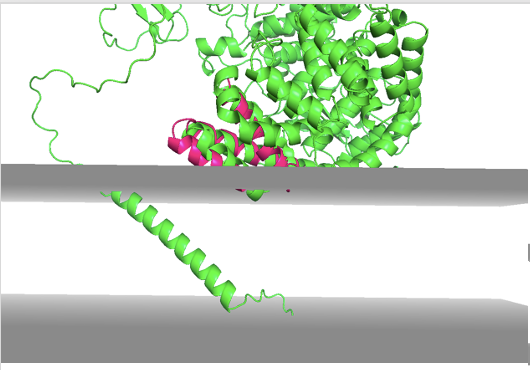
\includegraphics[width=\linewidth]{Pfam/Q6Q4G3.png}
  \caption{Aminopeptidase Q (Q6Q4G3) }
  \label{fig:q6q}
\end{subfigure}\hfil % <-- added
\begin{subfigure}{0.3\textwidth}
  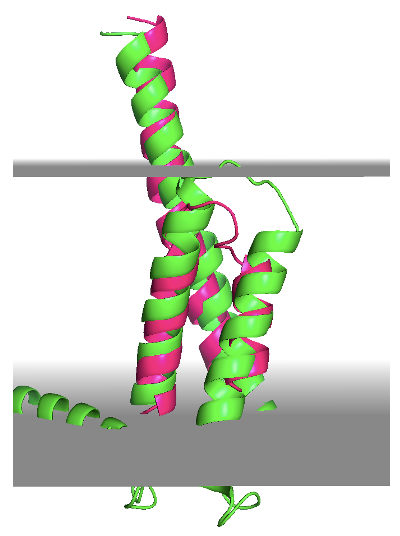
\includegraphics[width=\linewidth]{Pfam/Q9BUV8.png}
  \caption{Respirasome 
complex assembly factor 1 (Q9BUV8) }
  \label{fig:q9b}
\end{subfigure}
\caption{Other false positive hits}
\small
\begin{flushleft}
a) Presence of Aminopeptidase Q (Q6Q4G3) (green) false positive re-entrant loop/TM helix motif in relation to membrane bi-layer. The query (Yqja N-terminal re-entrant loop/TM helix motif) is shown in magenta. b) Presence of Respirasome 
complex assembly factor 1 (Q9BUV8) (green) re-entrant loop/TM helix motif in relation to membrane bilayer. The query (Yqja N-terminal re-entrant loop/TM helix motif) is shown in magenta.
\end{flushleft}

\label{fig:other_false_hits}
\end{figure}

The remaining nine models possessing the re-entrant loop/TM helix motif within the membrane bi-layer included three self hits with the human DedA homologues (Figure \ref{fig:selfhits}) as well as hits with transmembrane membrane proteins already known to possess the query structural motifs; Na\textsuperscript{+} transporters, Cl\textsuperscript{-} transporters and members of the Solute carrier family 13 (see Chapter 6). 

\begin{figure}[th!]
    \centering
    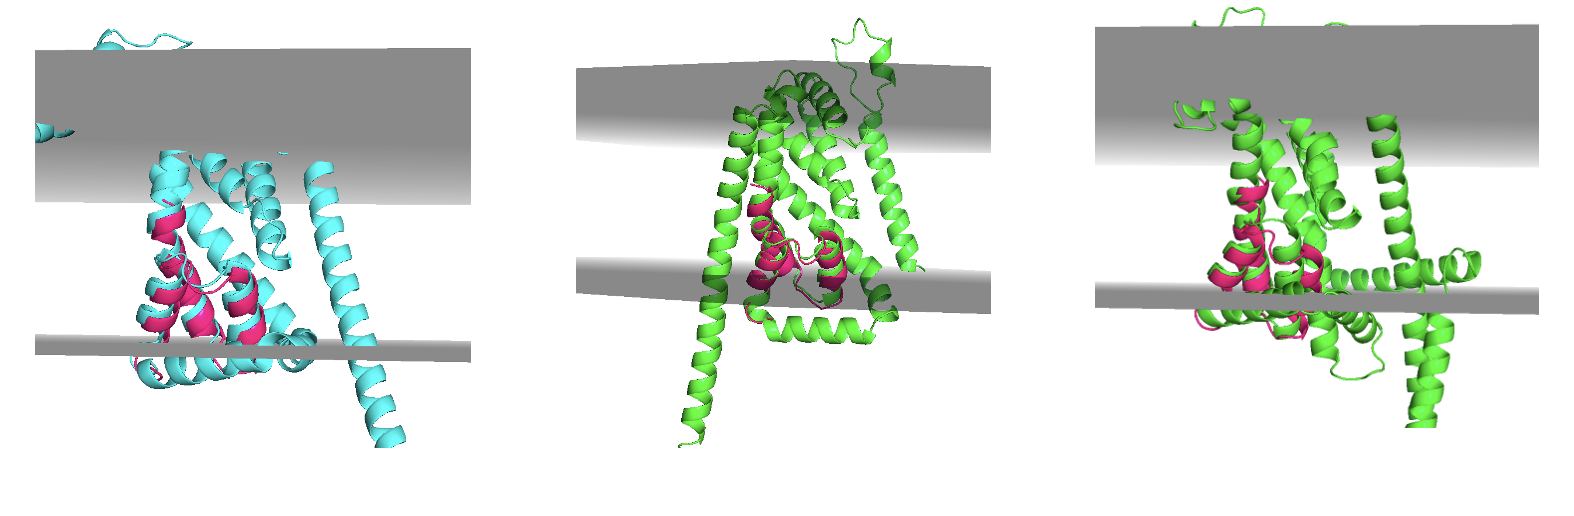
\includegraphics[width=150mm, scale=0.75]{Pfam/self_hits.png}
    \caption{Query DedA re-entrant loop/TM helix motif self hits}
    \label{fig:selfhits}
    \small
   \begin{flushleft}
 Query C-terminal re-entrant loop/TM helix motif from Tmem41b structurally alignments with (from left to right): Tmem41b, Tmem41a, Vmp1.\end{flushleft}

\end{figure}

In summary the screening of the DedA re-entrant loop/TM helix motif against the human AlphaFold database was able to identify known proteins that possess this structural motif.  Additionally, the screen also identified a hit that (Oca2) that is not known to have this structural feature.  Chapter 6 describes a detailed analysis of the predicted structure for Oca2 which contradicts the prevailing consensus topology of this physiological important protein. 
\iffalse

\fi



\section{Atg9 re-entrant AlphaFold Database Screen}

Atg9 possesses two re-entrant loops that have a structural role forming a kinked surface that contributes to the formation of a triangular wedge that acts as the inter-chain interface between each member of the trimer. The kinks of these re-entrant loops are formed by highly conserved proline residues, Pro302 in the N-terminal and Pro483 in C-terminal re-entrant loops \cite{guardia2020structure}.   These unusual re-entrant loops have not been recorded previously.  In an effort to identify other proteins that potentially possess these atypical structural features; the N-terminal re-entrant loop (residues 274-322) was extracted (Figure \ref{fig:atg9_rent}) and screened using the Dali server against the Human AlphaFold database. 

\begin{figure}[th!]
    \centering
    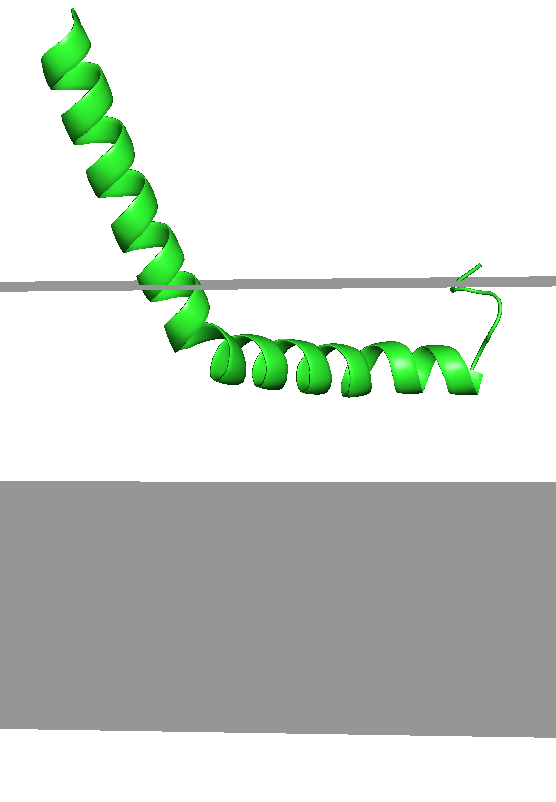
\includegraphics[width=75mm, scale=0.75]{Pfam/atg9_rent.png}
    \caption{Atg9 re-entrant isolated loop from CryoEM model with membrane planes}
    \label{fig:atg9_rent}
    \small
\end{figure}

The hits from the Dali results (Table  \ref{Table:dali_atg9_rent}) showed little consistency in terms of the classes and functions of the proteins.  The hits did not include the expected self-hit for Atg9.  In order to investigate the lack of self hits from the human AlphaFold database screen a pairwise Dali structural alignment was performed between the re-entrant loop in question and the Atg9 protein from which it was extracted.  Surprisingly Dali could not structurally align the two.  The inability of Dali being able to align the two structures possibly indicates some kind of limitation in the Dali software itself.  

Screening the hits generated by the Atg9 re-entrant loop screen by visually inspecting the structural alignments relative to the positioning of the membrane bilayer provided by the OMP server showed that even though accurate structural hits were obtained, they were not re-entrant loop structures.


\begin{table}[]
\caption{Dali results for structural screen of the Atg9 Re-entrant loop (Z-scores above 4.0)}
\resizebox{\columnwidth}{!}{%
\centering
\begin{tabular}{cl}
\rowcolor[HTML]{C65911} 
\multicolumn{1}{l}{\cellcolor[HTML]{C65911}Z-Score} & Hit Name                                                                 \\
\rowcolor[HTML]{FCE4D6} 
4.8                                                 & HUMAN:AF-Q15051-F1 IQ CALMODULIN-BINDING MOTIF-CONTAINING PROTEIN 1;     \\
\rowcolor[HTML]{F8CBAD} 
4.7                                                 & HUMAN:AF-P55081-F1 MICROFIBRILLAR-ASSOCIATED PROTEIN 1;                  \\
\rowcolor[HTML]{FCE4D6} 
4.7                                                 & HUMAN:AF-Q03135-F1 CAVEOLIN-1;                                           \\
\rowcolor[HTML]{F8CBAD} 
4.7                                                 & HUMAN:AF-Q7Z7H8-F1 39S RIBOSOMAL PROTEIN L10, MITOCHONDRIAL;             \\
\rowcolor[HTML]{FCE4D6} 
4.6                                                 & HUMAN:AF-Q9H307-F1 PININ;                                                \\
\rowcolor[HTML]{F8CBAD} 
4.6                                                 & HUMAN:AF-Q8IWA5-F1 CHOLINE TRANSPORTER-LIKE PROTEIN 2;                   \\
\rowcolor[HTML]{FCE4D6} 
4.6                                                 & HUMAN:AF-H3BTG2-F1 TESTIS-EXPRESSED PROTEIN 46;                          \\
\rowcolor[HTML]{F8CBAD} 
4.6                                                 & HUMAN:AF-Q96FZ7-F1 CHARGED MULTIVESICULAR BODY PROTEIN 6;                \\
\rowcolor[HTML]{FCE4D6} 
4.6                                                 & HUMAN:AF-Q9NST1-F1 1-ACYLGLYCEROL-3-PHOSPHATE O-ACYLTRANSFERASE PNPL     \\
\rowcolor[HTML]{F8CBAD} 
4.6                                                 & HUMAN:AF-Q9NS69-F1 MITOCHONDRIAL IMPORT RECEPTOR SUBUNIT TOM22 HOMOL     \\
\rowcolor[HTML]{FCE4D6} 
4.6                                                 & HUMAN:AF-Q8IVF4-F14 DYNEIN HEAVY CHAIN 10, AXONEMAL;                     \\
\rowcolor[HTML]{F8CBAD} 
4.6                                                 & HUMAN:AF-Q8NCM8-F11 CYTOPLASMIC DYNEIN 2 HEAVY CHAIN 1;                  \\
\rowcolor[HTML]{FCE4D6} 
4.5                                                 & HUMAN:AF-P04233-F1 HLA CLASS II HISTOCOMPATIBILITY ANTIGEN GAMMA CHANNEL \\
\rowcolor[HTML]{F8CBAD} 
4.5                                                 & HUMAN:AF-Q8IZT6-F11 ABNORMAL SPINDLE-LIKE MICROCEPHALY-ASSOCIATED PRO    \\
\rowcolor[HTML]{FCE4D6} 
4.5                                                 & HUMAN:AF-Q9UNK0-F1 SYNTAXIN-8;                                           \\
\rowcolor[HTML]{F8CBAD} 
4.4                                                 & HUMAN:AF-O00471-F1 EXOCYST COMPLEX COMPONENT 5;                          \\
\rowcolor[HTML]{FCE4D6} 
4.4                                                 & HUMAN:AF-Q8TE73-F13 DYNEIN HEAVY CHAIN 5, AXONEMAL;                      \\
\rowcolor[HTML]{F8CBAD} 
4.4                                                 & HUMAN:AF-O75154-F1 RAB11 FAMILY-INTERACTING PROTEIN 3;                   \\
\rowcolor[HTML]{FCE4D6} 
4.4                                                 & HUMAN:AF-P55268-F1 LAMININ SUBUNIT BETA-2;                               \\
\rowcolor[HTML]{F8CBAD} 
4.4                                                 & HUMAN:AF-Q96T54-F1 POTASSIUM CHANNEL SUBFAMILY K MEMBER 17;              \\
\rowcolor[HTML]{FCE4D6} 
4.3                                                 & HUMAN:AF-Q9H3R5-F1 CENTROMERE PROTEIN H;                                 \\
\rowcolor[HTML]{F8CBAD} 
4.3                                                 & HUMAN:AF-P56817-F1 BETA-SECRETASE 1;                                     \\
\rowcolor[HTML]{FCE4D6} 
4.3                                                 & HUMAN:AF-Q7Z419-F1 E3 UBIQUITIN-PROTEIN LIGASE RNF144B;                  \\
\rowcolor[HTML]{F8CBAD} 
4.3                                                 & HUMAN:AF-P24043-F6 LAMININ SUBUNIT ALPHA-2;                              \\
\rowcolor[HTML]{FCE4D6} 
4.2                                                 & HUMAN:AF-Q8TC41-F1 PROBABLE E3 UBIQUITIN-PROTEIN LIGASE RNF217;          \\
\rowcolor[HTML]{F8CBAD} 
4.2                                                 & HUMAN:AF-Q9BZF9-F1 UVEAL AUTOANTIGEN WITH COILED-COIL DOMAINS            \\
\rowcolor[HTML]{FCE4D6} 
4.2                                                 & HUMAN:AF-Q9UIF8-F1 BROMODOMAIN ADJACENT TO ZINC FINGER DOMAIN PROTEI     \\
\rowcolor[HTML]{F8CBAD} 
4.2                                                 & HUMAN:AF-Q5VIR6-F1 VACUOLAR PROTEIN SORTING-ASSOCIATED PROTEIN 53 HO     \\
\rowcolor[HTML]{FCE4D6} 
4.2                                                 & HUMAN:AF-Q8WXX0-F8 DYNEIN HEAVY CHAIN 7, AXONEMAL;                       \\
\rowcolor[HTML]{F8CBAD} 
4.2                                                 & HUMAN:AF-Q0VDD8-F7 DYNEIN HEAVY CHAIN 14, AXONEMAL;                      \\
\rowcolor[HTML]{FCE4D6} 
4.1                                                 & HUMAN:AF-P06127-F1 T-CELL SURFACE GLYCOPROTEIN CD5;                      \\
\rowcolor[HTML]{F8CBAD} 
4.1                                                 & HUMAN:AF-Q9Y6N6-F1 LAMININ SUBUNIT GAMMA-3;                              \\
\rowcolor[HTML]{FCE4D6} 
4.1                                                 & HUMAN:AF-Q93074-F1 MEDIATOR OF RNA POLYMERASE II TRANSCRIPTION SUBUN     \\
\rowcolor[HTML]{F8CBAD} 
4.1                                                 & HUMAN:AF-Q9NQ34-F1 TRANSMEMBRANE PROTEIN 9B;                             \\
\rowcolor[HTML]{FCE4D6} 
4.1                                                 & HUMAN:AF-Q14207-F1 PROTEIN NPAT;                                         \\
\rowcolor[HTML]{F8CBAD} 
4.1                                                 & HUMAN:AF-Q6TFL3-F1 COILED-COIL DOMAIN-CONTAINING PROTEIN 171;            \\
\rowcolor[HTML]{FCE4D6} 
4.1                                                 & HUMAN:AF-P02679-F1 FIBRINOGEN GAMMA CHAIN;                               \\
\rowcolor[HTML]{F8CBAD} 
4.1                                                 & HUMAN:AF-Q9UI33-F1 SODIUM CHANNEL PROTEIN TYPE 11 SUBUNIT ALPHA;        
\end{tabular}
}
\label{Table:dali_atg9_rent}
\end{table}


A more detailed inspection of the membrane channel hits was conducted as the re-entrant loop query originated from a putative channel protein. Slc44a2 controls platelet activation and thrombosis  mediating choline conductance across the mitochodrial membrane thereby regulating mitochondrial energetics \cite{bennett2020choline}. It can be seen in Figure \ref{fig:atg9_rent_hit} that the aligned region of the target does possess the correct fold but is not positioned in the membrane bi-layer. 


\begin{figure}[th!]
    \centering
    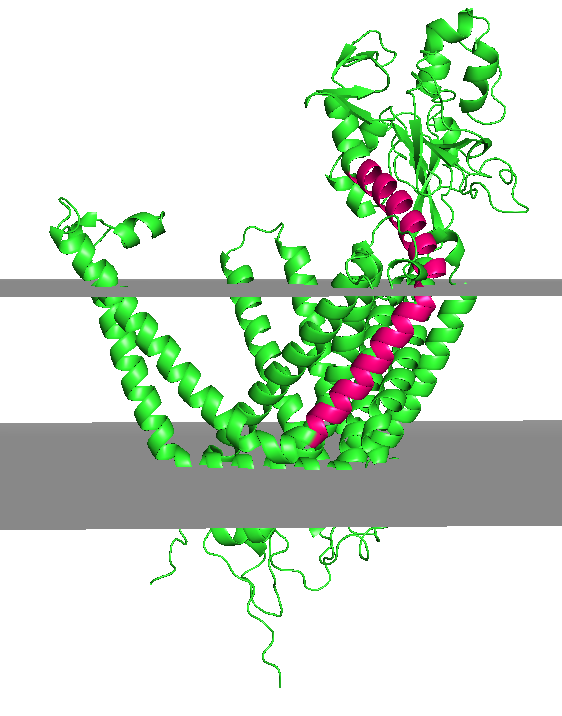
\includegraphics[width=75mm, scale=0.75]{Pfam/atg9_rent aln.png}
    \caption{Human SCL44A2 AlphaFold2 model with Magenta highlighting Atg9 re-entrant alignment region.}
    \label{fig:atg9_rent_hit}
    \small
\end{figure}

The simplicity of the re-entrant loop structure is probably responsible for the absence of any positive structural hits for these unusual structural features. A search involving the alignment of the Atg9 re-entrant loop with additional structural features (upstream and/or downstream from the re-entrant loop) could possibly yield structural hits when this kind of mining exercise with simple structural regions is performed. Structural information coupled with, for example, hydrophobic distribution would provided additional mining criteria to identify equivalent structural regions from a large database.  In terms of the specific Atg9 re-entrant loop; it could also be that this feature is unique to Atg9.


\section{Conclusions}
Large complex transmembrane proteins can be successfully be modelled with AlphaFold2.  The models can be used to infer homology in the absence of any detectable sequence similarity.  This can be seen, for example, the strong structural alignments between representative models of PF00230, PF10136 and PF01226.  Additionally, these highly accurate structural predictions made by AlphaFold2 can be mined to identify proteins possessing sub-structures of interest.  The presence of specific sub-structures can infer function of these proteins. Screening for simple sub-structures such as the Atg9 re-entrant loop proved difficult.  However, screening both a transmembrane Pfam model library as well as the human AlphaFold database for a more complex sub-structure such as the  re-entrant loop/transmembrane helix motif proved more successful resulting in identifying proteins possessing the re-entrant loop/transmembrane helix motif; as a result, the function of these proteins were inferred confidently (see chapter 6 for the in depth analysis of Oca2).  






